%%%%%%%%%%%%%%%%%%%%%%%%%%%%%%%%%%%%%%%%%
%  A bright and image filled report style, currently set up here for use with ILM report 8600-219.
%  Contains all that is required, glossaries, content management, references and good looks.
%
% The original template (the Legrand Orange Book Template) can be found here --> http://www.latextemplates.com/template/the-legrand-orange-book
% Original author of the Legrand Orange Book Template:
% Mathias Legrand (legrand.mathias@gmail.com) 
%
% Modifications made for ILM specific reporting
% 
%
% License:
% CC BY-NC-SA 3.0 (http://creativecommons.org/licenses/by-nc-sa/3.0/)
%%%%%%%%%%%%%%%%%%%%%%%%%%%%%%%%%%%%%%%%%
 
%%%%%%%%%%%%%%%%%%%%%%%%%%%%%%%%%%%%%%%%%
% How to use this
%
% Upload a file called FrontCover.jpg to become your new front cover - into the Pictures folder
% Upload files called Heading1.jpg, Heading2.jpg etc to become your new chapter headers - into the Pictures folder
% Make sure these images are the right size to fit their locations and use good quality images
%
% Locate the variables below and set your name, title etc.
%
% If you want to change text colour on the front cover, the areas required are commented below
% If you want to modify text and border colours for your chapter headers go into the structure.tex file and replace the name of the colour (set to ) with a new colour name (find and replace ctrl+f will do this for you).
%
% Add all references into references.bib
% Cite these references by using \cite{referenceName}
%
% Commonly used acronyms or industry specific terms should be added to the glossary
% These terms may then be referenced in the text using \gls{termName}
%
% Finally put some answers in there!
%
% 
% Note: This template is set up specifically for ILM reports, it can be modified for other forms of reports
%
%%%%%%%%%%%%%%%%%%%%%%%%%%%%%%%%%%%%%%%%
 
 
%----------------------------------------------------------------------------------------
%	SET THESE VARIABLES!
%----------------------------------------------------------------------------------------

\def\mytitle{ Vectorial Calculus } % Title of the ILM project
\def\ILMCode{Adbridged, it seems.} % Unique code for the ILM project

\def\author{Jaime Andres Torres B.} % Your name.. 
\def\id{github.com/XaurDesu} % Your unique identifier

\def\date{\today } % Today's date 


 
%----------------------------------------------------------------------------------------
%	PACKAGES AND OTHER DOCUMENT CONFIGURATIONS
%----------------------------------------------------------------------------------------

\documentclass[11pt,fleqn]{book} % Default font size and left-justified equations

\usepackage[dvipsnames]{xcolor}

%%%%%%%%%%%%%%%%%%%%%%%%%%%%%%%%%%%%%%%%%
% This is based on the Legrand Orange Book
% Structural Definitions File
%
% The original template (the Legrand Orange Book Template) can be found here --> http://www.latextemplates.com/template/the-legrand-orange-book
%
% Original author of the Legrand Orange Book Template::
% Mathias Legrand (legrand.mathias@gmail.com) with modifications by:
% Vel (vel@latextemplates.com)
%
% Original License:
% CC BY-NC-SA 3.0 (http://creativecommons.org/licenses/by-nc-sa/3.0/)
%
%%%%%%%%%%%%%%%%%%%%%%%%%%%%%%%%%%%%%%%%%
%----------------------------------------------------------------------------------------
%	VARIOUS REQUIRED PACKAGES
%----------------------------------------------------------------------------------------

\usepackage{titlesec} % Allows customization of titles

\usepackage{graphicx} % Required for including pictures
\graphicspath{{Pictures/}} % Specifies the directory where pictures are stored

\usepackage{lipsum} % Inserts dummy text

\usepackage{tikz} % Required for drawing custom shapes

\usepackage[english]{babel} % English language/hyphenation

\usepackage{enumitem} % Customize lists

\setlist{nolistsep} % Reduce spacing between bullet points and numbered lists

\usepackage{booktabs} % Required for nicer horizontal rules in tables

\usepackage{eso-pic} % Required for specifying an image background in the title page

\usepackage{glossaries} %Required to allow the creation of glossary items, allows for referencing within the document

\usepackage[none]{hyphenat} %Stops words which are too long for a line being split over two lines using hyphenation

\usepackage[top=3cm,bottom=3cm,left=3.2cm,right=3.2cm,headsep=10pt,letterpaper]{geometry} % Page margins
\usepackage{algorithm} % Writing nice algorithms
\usepackage{algpseudocode} % Writing pseudocode
\usepackage{longtable} %Tables which may stretch over more than 1 page
\usepackage{rotating} %Rotate images using sideswaysimage


% Font Settings
\usepackage{avant} % Use the Avantgarde font for headings
%\usepackage{times} % Use the Times font for headings
\usepackage{mathptmx} % Use the Adobe Times Roman as the default text font together with math symbols from the Symbol, Chancery and Computer Modern fonts

\usepackage{microtype} % Slightly tweak font spacing for aesthetics
\usepackage[utf8]{inputenc} % Required for including letters with accents
\usepackage[T1]{fontenc} % Use 8-bit encoding that has 256 glyphs

%----------------------------------------------------------------------------------------
%	MAIN TABLE OF CONTENTS
%----------------------------------------------------------------------------------------

\usepackage{titletoc} % Required for manipulating the table of contents

\contentsmargin{0cm} % Removes the default margin
% Chapter text styling
\titlecontents{chapter}[1.25cm] % Indentation
{\addvspace{15pt}\large\sffamily\bfseries} % Spacing and font options for chapters
{\color{Apricot!60}\contentslabel[\Large\thecontentslabel]{1.25cm}\color{Apricot}} % Chapter number
{}  
{\color{Apricot!60}\normalsize\sffamily\bfseries\;\titlerule*[.5pc]{.}\;\thecontentspage} % Page number
% Section text styling
\titlecontents{section}[1.25cm] % Indentation
{\addvspace{5pt}\sffamily\bfseries} % Spacing and font options for sections
{\contentslabel[\thecontentslabel]{1.25cm}} % Section number
{}
{\sffamily\hfill\color{black}\thecontentspage} % Page number
[]
% Subsection text styling
\titlecontents{subsection}[1.25cm] % Indentation
{\addvspace{1pt}\sffamily\small} % Spacing and font options for subsections
{\contentslabel[\thecontentslabel]{1.25cm}} % Subsection number
{}
{\sffamily\;\titlerule*[.5pc]{.}\;\thecontentspage} % Page number
[] 

%----------------------------------------------------------------------------------------
%	MINI TABLE OF CONTENTS IN CHAPTER HEADS
%----------------------------------------------------------------------------------------

% Section text styling
\titlecontents{lsection}[0em] % Indendating
{\footnotesize\sffamily} % Font settings
{}
{}
{}

% Subsection text styling
\titlecontents{lsubsection}[.5em] % Indentation
{\normalfont\footnotesize\sffamily} % Font settings
{}
{}
{}
 
%----------------------------------------------------------------------------------------
%	PAGE HEADERS
%----------------------------------------------------------------------------------------

\usepackage{fancyhdr} % Required for header and footer configuration

\pagestyle{fancy}
\renewcommand{\chaptermark}[1]{\markboth{\sffamily\normalsize\bfseries\chaptername\ \thechapter.\ #1}{}} % Chapter text font settings
\renewcommand{\sectionmark}[1]{\markright{\sffamily\normalsize\thesection\hspace{5pt}#1}{}} % Section text font settings
\fancyhf{} \fancyhead[LE,RO]{\sffamily\normalsize\thepage} % Font setting for the page number in the header
\fancyhead[LO]{\rightmark} % Print the nearest section name on the left side of odd pages
\fancyhead[RE]{\leftmark} % Print the current chapter name on the right side of even pages
\renewcommand{\headrulewidth}{0.5pt} % Width of the rule under the header
\addtolength{\headheight}{2.5pt} % Increase the spacing around the header slightly
\renewcommand{\footrulewidth}{0pt} % Removes the rule in the footer
\fancypagestyle{plain}{\fancyhead{}\renewcommand{\headrulewidth}{0pt}} % Style for when a plain pagestyle is specified

% Removes the header from odd empty pages at the end of chapters
\makeatletter
\renewcommand{\cleardoublepage}{
\clearpage\ifodd\c@page\else
\hbox{}
\vspace*{\fill}
\thispagestyle{empty}
\newpage
\fi}

%----------------------------------------------------------------------------------------
%	THEOREM STYLES
%----------------------------------------------------------------------------------------

\usepackage{amsmath,amsfonts,amssymb,amsthm} % For math equations, theorems, symbols, etc

\newcommand{\intoo}[2]{\mathopen{]}#1\,;#2\mathclose{[}}
\newcommand{\ud}{\mathop{\mathrm{{}d}}\mathopen{}}
\newcommand{\intff}[2]{\mathopen{[}#1\,;#2\mathclose{]}}
\newtheorem{notation}{Notation}[chapter]

%%%%%%%%%%%%%%%%%%%%%%%%%%%%%%%%%%%%%%%%%%%%%%%%%%%%%%%%%%%%%%%%%%%%%%%%%%%
%%%%%%%%%%%%%%%%%%%% dedicated to boxed/framed environements %%%%%%%%%%%%%%
%%%%%%%%%%%%%%%%%%%%%%%%%%%%%%%%%%%%%%%%%%%%%%%%%%%%%%%%%%%%%%%%%%%%%%%%%%%
\newtheoremstyle{Orchidnumbox}% % Theorem style name
{0pt}% Space above
{0pt}% Space below
{\normalfont}% % Body font
{}% Indent amount
{\small\bf\sffamily\color{Apricot}}% % Theorem head font
{\;}% Punctuation after theorem head
{0.25em}% Space after theorem head
{\small\sffamily\color{Apricot}\thmname{#1}\nobreakspace\thmnumber{\@ifnotempty{#1}{}\@upn{#2}}% Theorem text (e.g. Theorem 2.1)
\thmnote{\nobreakspace\the\thm@notefont\sffamily\bfseries\color{black}---\nobreakspace#3.}} % Optional theorem note
\renewcommand{\qedsymbol}{$\blacksquare$}% Optional qed square

\newtheoremstyle{blacknumex}% Theorem style name
{5pt}% Space above
{5pt}% Space below
{\normalfont}% Body font
{} % Indent amount
{\small\bf\sffamily}% Theorem head font
{\;}% Punctuation after theorem head
{0.25em}% Space after theorem head
{\small\sffamily{\tiny\ensuremath{\blacksquare}}\nobreakspace\thmname{#1}\nobreakspace\thmnumber{\@ifnotempty{#1}{}\@upn{#2}}% Theorem text (e.g. Theorem 2.1)
\thmnote{\nobreakspace\the\thm@notefont\sffamily\bfseries---\nobreakspace#3.}}% Optional theorem note

\newtheoremstyle{blacknumbox} % Theorem style name
{0pt}% Space above
{0pt}% Space below
{\normalfont}% Body font
{}% Indent amount
{\small\bf\sffamily}% Theorem head font
{\;}% Punctuation after theorem head
{0.25em}% Space after theorem head
{\small\sffamily\thmname{#1}\nobreakspace\thmnumber{\@ifnotempty{#1}{}\@upn{#2}}% Theorem text (e.g. Theorem 2.1)
\thmnote{\nobreakspace\the\thm@notefont\sffamily\bfseries---\nobreakspace#3.}}% Optional theorem note

%%%%%%%%%%%%%%%%%%%%%%%%%%%%%%%%%%%%%%%%%%%%%%%%%%%%%%%%%%%%%%%%%%%%%%%%%%%
%%%%%%%%%%%%% dedicated to non-boxed/non-framed environements %%%%%%%%%%%%%
%%%%%%%%%%%%%%%%%%%%%%%%%%%%%%%%%%%%%%%%%%%%%%%%%%%%%%%%%%%%%%%%%%%%%%%%%%%
\newtheoremstyle{Orchidnum}% % Theorem style name
{5pt}% Space above
{5pt}% Space below
{\normalfont}% % Body font
{}% Indent amount
{\small\bf\sffamily\color{Apricot}}% % Theorem head font
{\;}% Punctuation after theorem head
{0.25em}% Space after theorem head
{\small\sffamily\color{Apricot}\thmname{#1}\nobreakspace\thmnumber{\@ifnotempty{#1}{}\@upn{#2}}% Theorem text (e.g. Theorem 2.1)
\thmnote{\nobreakspace\the\thm@notefont\sffamily\bfseries\color{black}---\nobreakspace#3.}} % Optional theorem note
\renewcommand{\qedsymbol}{$\blacksquare$}% Optional qed square
\makeatother

% Defines the theorem text style for each type of theorem to one of the three styles above
\newcounter{dummy} 
\numberwithin{dummy}{section}
\theoremstyle{Orchidnumbox}
\newtheorem{theoremeT}[dummy]{Theorem}
\newtheorem{problem}{Problem}[chapter]
\newtheorem{exerciseT}{Exercise}[chapter]
\theoremstyle{blacknumex}
\newtheorem{exampleT}{Example}[chapter]
\theoremstyle{blacknumbox}
\newtheorem{vocabulary}{Vocabulary}[chapter]
\newtheorem{definitionT}{Definition}[section]
\newtheorem{corollaryT}[dummy]{Corollary}
\theoremstyle{Orchidnum}
\newtheorem{proposition}[dummy]{Proposition}

%----------------------------------------------------------------------------------------
%	DEFINITION OF COLORED BOXES
%----------------------------------------------------------------------------------------

\RequirePackage[framemethod=default]{mdframed} % Required for creating the theorem, definition, exercise and corollary boxes

% Theorem box
\newmdenv[skipabove=7pt,
skipbelow=7pt,
backgroundcolor=black!5,
linecolor= Apricot, % Modify the colour of theorem boxes
innerleftmargin=5pt,
innerrightmargin=5pt,
innertopmargin=5pt,
leftmargin=0cm,
rightmargin=0cm,
innerbottommargin=5pt]{tBox}

% Exercise box	  
\newmdenv[skipabove=7pt,
skipbelow=7pt,
rightline=false,
leftline=true,
topline=false,
bottomline=false,
backgroundcolor=Apricot!10,
linecolor=Apricot,
innerleftmargin=5pt,
innerrightmargin=5pt,
innertopmargin=5pt,
innerbottommargin=5pt,
leftmargin=0cm,
rightmargin=0cm,
linewidth=4pt]{eBox}	

% Definition box
\newmdenv[skipabove=7pt,
skipbelow=7pt,
rightline=false,
leftline=true,
topline=false,
bottomline=false,
linecolor=Apricot,
innerleftmargin=5pt,
innerrightmargin=5pt,
innertopmargin=0pt,
leftmargin=0cm,
rightmargin=0cm,
linewidth=4pt,
innerbottommargin=0pt]{dBox}	

% Corollary box
\newmdenv[skipabove=7pt,
skipbelow=7pt,
rightline=false,
leftline=true,
topline=false,
bottomline=false,
linecolor=gray,
backgroundcolor=black!5,
innerleftmargin=5pt,
innerrightmargin=5pt,
innertopmargin=5pt,
leftmargin=0cm,
rightmargin=0cm,
linewidth=4pt,
innerbottommargin=5pt]{cBox}

% Creates an environment for each type of theorem and assigns it a theorem text style from the "Theorem Styles" section above and a colored box from above
\newenvironment{theorem}{\begin{tBox}\begin{theoremeT}}{\end{theoremeT}\end{tBox}}
\newenvironment{exercise}{\begin{eBox}\begin{exerciseT}}{\hfill{\color{Apricot}\tiny\ensuremath{\blacksquare}}\end{exerciseT}\end{eBox}}				  
\newenvironment{definition}{\begin{dBox}\begin{definitionT}}{\end{definitionT}\end{dBox}}	
\newenvironment{example}{\begin{exampleT}}{\hfill{\tiny\ensuremath{\blacksquare}}\end{exampleT}}		
\newenvironment{corollary}{\begin{cBox}\begin{corollaryT}}{\end{corollaryT}\end{cBox}}	

%----------------------------------------------------------------------------------------
%	REMARK ENVIRONMENT
%----------------------------------------------------------------------------------------

\newenvironment{remark}{\par\vspace{10pt}\small % Vertical white space above the remark and smaller font size
\begin{list}{}{
\leftmargin=35pt % Indentation on the left
\rightmargin=25pt}\item\ignorespaces % Indentation on the right
\makebox[-2.5pt]{\begin{tikzpicture}[overlay]
\node[draw=Orchid!60,line width=1pt,circle,fill=Orchid!25,font=\sffamily\bfseries,inner sep=2pt,outer sep=0pt] at (-15pt,0pt){\textcolor{Apricot}{R}};\end{tikzpicture}} % Orange R in a circle
\advance\baselineskip -1pt}{\end{list}\vskip5pt} % Tighter line spacing and white space after remark

%----------------------------------------------------------------------------------------
%	SECTION NUMBERING IN THE MARGIN
%----------------------------------------------------------------------------------------

\makeatletter
\renewcommand{\@seccntformat}[1]{\llap{\textcolor{Apricot}{\csname the#1\endcsname}\hspace{1em}}}                    
\renewcommand{\section}{\@startsection{section}{1}{\z@}
{-4ex \@plus -1ex \@minus -.4ex}
{1ex \@plus.2ex }
{\normalfont\large\sffamily\bfseries}}
\renewcommand{\subsection}{\@startsection {subsection}{2}{\z@}
{-3ex \@plus -0.1ex \@minus -.4ex}
{0.5ex \@plus.2ex }
{\normalfont\sffamily\bfseries}}
\renewcommand{\subsubsection}{\@startsection {subsubsection}{3}{\z@}
{-2ex \@plus -0.1ex \@minus -.2ex}
{.2ex \@plus.2ex }
{\normalfont\small\sffamily\bfseries}}                        
\renewcommand\paragraph{\@startsection{paragraph}{4}{\z@}
{-2ex \@plus-.2ex \@minus .2ex}
{.1ex}
{\normalfont\small\sffamily\bfseries}}

%----------------------------------------------------------------------------------------
%	HYPERLINKS IN THE DOCUMENTS
%----------------------------------------------------------------------------------------

% For an unclear reason, the package should be loaded now and not later
\usepackage{hyperref}
\hypersetup{hidelinks,colorlinks=false,breaklinks=true,urlcolor= Orchid,bookmarksopen=false,pdftitle={Title},pdfauthor={Author}}

%----------------------------------------------------------------------------------------
%	CHAPTER HEADINGS
%----------------------------------------------------------------------------------------

% The set-up below should be (sadly) manually adapted to the overall margin page septup controlled by the geometry package loaded in the main.tex document. It is possible to implement below the dimensions used in the goemetry package (top,bottom,left,right)... TO BE DONE

\newcommand{\thechapterimage}{}
\newcommand{\chapterimage}[1]{\renewcommand{\thechapterimage}{#1}}

% Numbered chapters with mini tableofcontents
\def\thechapter{\arabic{chapter}}
\def\@makechapterhead#1{
\thispagestyle{empty}
{\centering \normalfont\sffamily
\ifnum \c@secnumdepth >\m@ne
\if@mainmatter
\startcontents
\begin{tikzpicture}[remember picture,overlay]
\node at (current page.north west)
{\begin{tikzpicture}[remember picture,overlay]
\node[anchor=north west,inner sep=0pt] at (0,0) {\includegraphics[width=\paperwidth]{\thechapterimage}};
%%%%%%%%%%%%%%%%%%%%%%%%%%%%%%%%%%%%%%%%%%%%%%%%%%%%%%%%%%%%%%%%%%%%%%%%%%%%%%%%%%%%%
% Commenting the 3 lines below removes the small contents box in the chapter heading
%\fill[color=Orchid!10!white,opacity=.6] (1cm,0) rectangle (8cm,-7cm);
%\node[anchor=north west] at (1.1cm,.35cm) {\parbox[t][8cm][t]{6.5cm}{\huge\bfseries\flushleft \printcontents{l}{1}{\setcounter{tocdepth}{2}}}};
\draw[anchor=west] (5cm,-9cm) node [rounded corners=20pt,fill=Apricot!10!white,text opacity=1,draw=Apricot,draw opacity=1,line width=1.5pt,fill opacity=.6,inner sep=12pt]{\huge\sffamily\bfseries\textcolor{black}{\thechapter. #1\strut\makebox[22cm]{}}};
%%%%%%%%%%%%%%%%%%%%%%%%%%%%%%%%%%%%%%%%%%%%%%%%%%%%%%%%%%%%%%%%%%%%%%%%%%%%%%%%%%%%%
\end{tikzpicture}};
\end{tikzpicture}}
\par\vspace*{230\p@}
\fi
\fi}

% Unnumbered chapters without mini tableofcontents (could be added though) 
\def\@makeschapterhead#1{
\thispagestyle{empty}
{\centering \normalfont\sffamily
\ifnum \c@secnumdepth >\m@ne
\if@mainmatter
\begin{tikzpicture}[remember picture,overlay]
\node at (current page.north west)
{\begin{tikzpicture}[remember picture,overlay]
\node[anchor=north west,inner sep=0pt] at (0,0) {\includegraphics[width=\paperwidth]{\thechapterimage}};
\draw[anchor=west] (5cm,-9cm) node [rounded corners=20pt,fill=Apricot!10!white,fill opacity=.6,inner sep=12pt,text opacity=1,draw=Apricot,draw opacity=1,line width=1.5pt]{\huge\sffamily\bfseries\textcolor{black}{#1\strut\makebox[22cm]{}}};
\end{tikzpicture}};
\end{tikzpicture}}
\par\vspace*{230\p@}
\fi
\fi
}
\makeatother % Insert the commands.tex file which contains the majority of the structure behind the template

\makeglossaries

%--------------------------------------------------------------------------

% Glossary entries

%--------------------------------------------------------------------------
\newglossaryentry{ETN}
{
    name = {Example Term Name (ETN)},
    description = {What does this term mean? Any examples of it? Further reading? References?}
}

%--------------------------------------------------------------------------

% Document begins here

%--------------------------------------------------------------------------

\begin{document}
\renewcommand{\bibname}{References} % Adds in the link to your references


%----------------------------------------------------------------------------------------
%	TITLE PAGE
%----------------------------------------------------------------------------------------

\begingroup
\thispagestyle{empty}
\AddToShipoutPicture*{\put(0,0){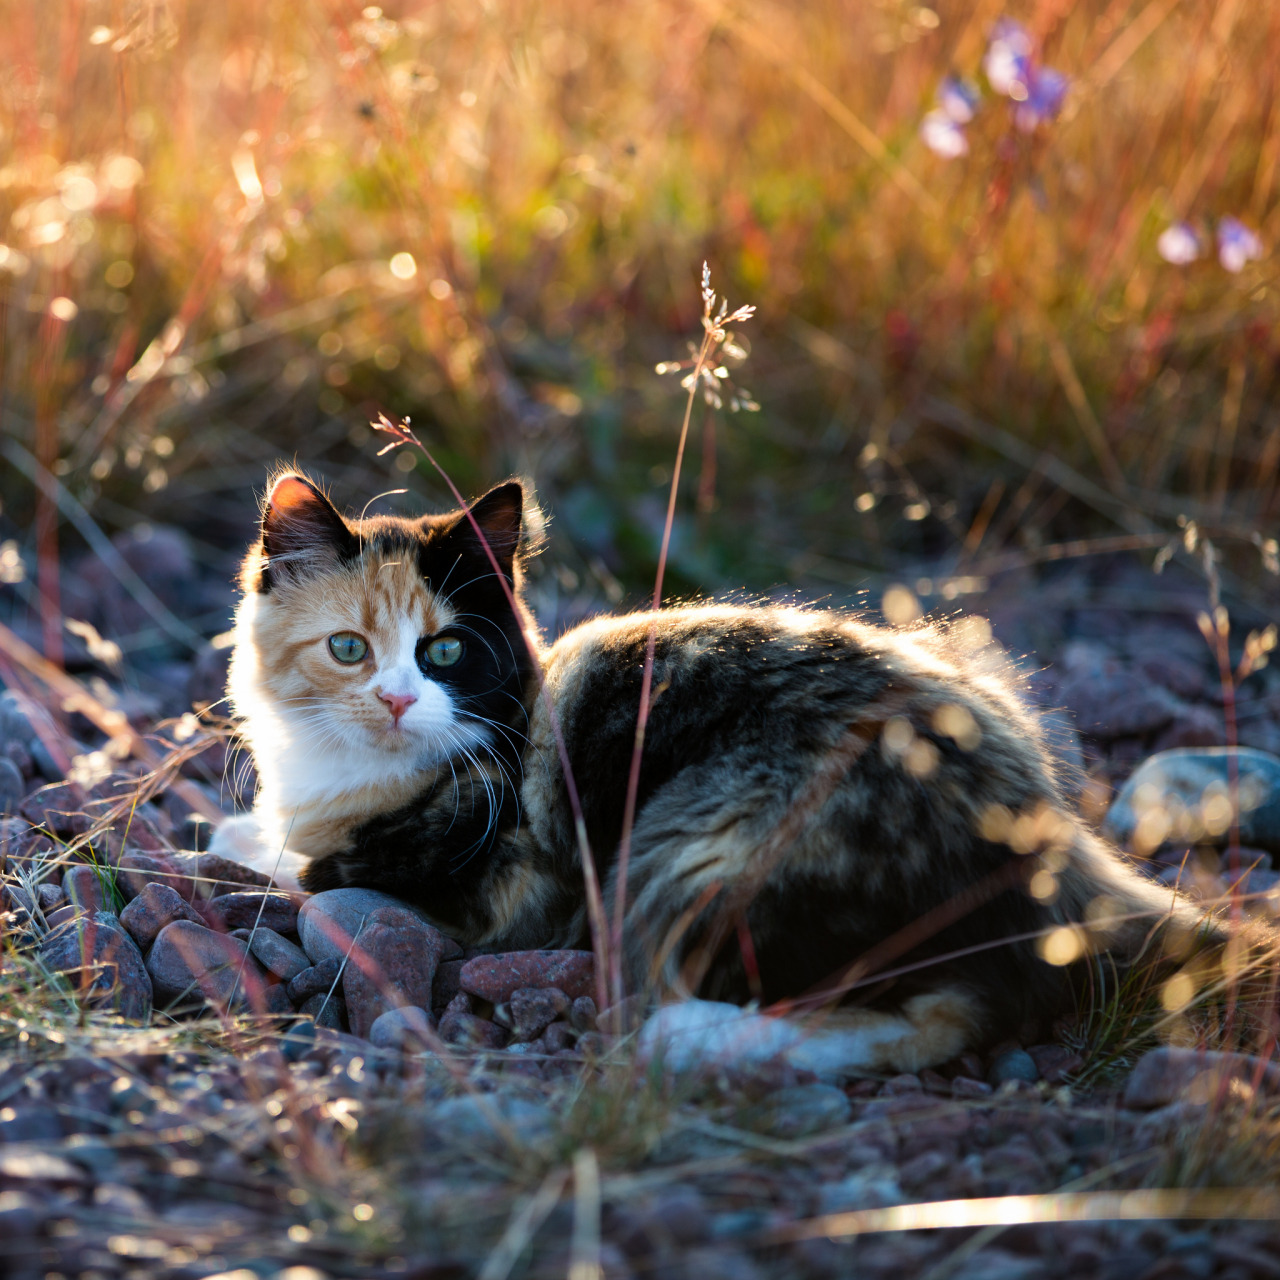
\includegraphics{Pictures/FrontCover.jpg}}} % Image background
\centering
\vspace*{11.3cm}
\par\normalfont\fontsize{35}{35}\sffamily\selectfont

\begin{center}
    % List of Latex Colour names here: https://www.overleaf.com/learn/latex/Using_colours_in_LaTeX
    \textbf{\color{Apricot} \mytitle}  % Modify the name of the colour used to suit your image
    
    \textbf{\color{White}(\ILMCode)} % Modify the name of the colour used to suit your image
    
    \color{white}Uniandes\par % Modify the name of the colour used to suit your image
    
    \vspace*{0.5cm}
    \color{Apricot}\author % Modify the name of the colour used to suit your image
    
    (\id)\par  
\end{center}

\endgroup

%----------------------------------------------------------------------------------------
%	COPYRIGHT PAGE
%----------------------------------------------------------------------------------------


\newpage
~\vfill
\thispagestyle{empty}

\noindent \textbf{Vectorial Calculus - }
\vspace{0.5cm}

\noindent 
\vspace{1cm}

\noindent \textit{First release, \date} % Printing/edition date

%----------------------------------------------------------------------------------------
%	TABLE OF CONTENTS
%----------------------------------------------------------------------------------------

\chapterimage{Heading1.jpg} % Table of contents heading image

\pagestyle{empty} % No headers

\tableofcontents % Print the table of contents itself

%\listoftables %uncomment this if you want to print the list of tables at the start

\pagestyle{fancy} % Print headers again


%----------------------------------------------------------------------------------------
%	Glossary
%----------------------------------------------------------------------------------------

\chapterimage{Heading1.jpg} % Table of contents heading image

\printglossaries



%----------------------------------------------------------------------------------------
%	First set of related questions
%----------------------------------------------------------------------------------------

\chapterimage{Heading2.jpg}
\chapter{Introduction}

\begin{flushright}
    \textit{Go big or go home.}
\end{flushright}

Vectorial calculus is what the title says pretty much, the act of using methods
proper to calculus on vectorial spaces, for the topic of this class generally referring to
merely 3-dimensional ones, at the end of this book you should be able to:

\begin{itemize}
    \item 
\end{itemize}

\vspace{20px}
\vspace{0.5cm} % Adds some vertical whitespace, easier to read

%--------------------------------------------------------------
%	More sections?
%----------------------------------------------------------------------------

\chapter{Linear Algebra Concepts}
\section{Vectors on a three-dimensional space.}

given an $ \mathbb{R}^3 $ space and a point in that space $ P = (a,b,c) $,
we can describe a vector by either connecting the point $ P $ to another point $ Q $, or
by assuming the origin of this space (point $ (0,0,0) $), this is a mathematical object with both a
direction and a magnitude. The direction is given by an angle and the 
magnitude is given by $\sqrt{a_1^2 + a_2^2 + a_3^2}$

As an example, let's assume the vector given by $ P = (1,2,1) $:
\begin{center}
    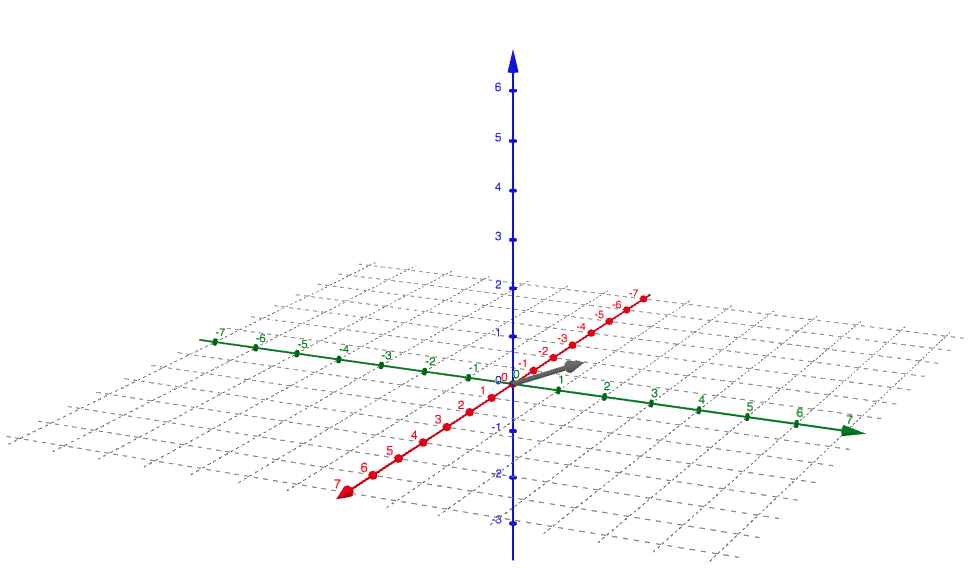
\includegraphics[scale=0.35]{vector_1.png}

    \textit{Vector formed by $ P = (1,2,1) $}
\end{center}

For this vector, we can calculate the magnitude by replacing the vectorial components by 
the magnitudes of the individual directions, resulting in:

%\begin{gather}
 %    \sqrt{1^2 + 2^2 + 1^2} \\
%
 %    \sqrt{1+4+1} \\
  %  
   %  \sqrt{6} \\
%\end{gather}

\textit{Note, in this course we will be mostly only concerned with }$ \mathbb{R}^3 $
\subsection{Addition and Subtraction}

We can take any $ \vec{a} $ and $ \vec{b} $ vectors on the same space and add them to each other
in the form:

\begin{equation}
    \begin{bmatrix}
        a_1 \\
        a_2 \\
        a_3 \\
    \end{bmatrix}
    +
    \begin{bmatrix}
        b_1 \\
        b_2 \\
        b_3 \\
    \end{bmatrix}
    = 
    \begin{pmatrix}
        a_1 + b_1\\
        a_2 + b_2\\
        a_3 + b_3\\
    \end{pmatrix}
\end{equation}

Such form remains in the case we can do subtraction, which is expressed on the equation:

\begin{equation}
    \begin{bmatrix}
        a_1 \\
        a_2 \\
        a_3 \\
    \end{bmatrix}
    -
    \begin{bmatrix}
        b_1 \\
        b_2 \\
        b_3 \\
    \end{bmatrix}
    = 
    \begin{pmatrix}
        a_1 - b_1\\
        a_2 - b_2\\
        a_3 - b_3\\
    \end{pmatrix}
\end{equation}

This kind of operations have certain properties, shown as:
\begin{gather}
    (\alpha + \beta)\vec[v] = \alpha\vec{v} + \beta\vec{v} \\
    \vec{v} * 1 = \vec{v} \\
    \vec{v} * \vec{0} = \vec{0} \\
    \beta \vec{v} = 
    \begin{pmatrix}
        \beta a_1\\
        \beta a_2\\
        \beta a_3\\
    \end{pmatrix}
\end{gather}

Two vectors $ \vec{a} $ and $ \vec{b} $ are equal if and only if:
\begin{equation}
    \begin{cases}
        \vec{a} \exists \mathbb{R}^3 \\
        \vec{b} \exists \mathbb{R}^3
    \end{cases}
    \implies
    \begin{pmatrix}
        a_1 = b_1\\
        a_2 = b_2\\
        a_3 = b_3\\
    \end{pmatrix}
    \text{
        \textit{note: this can be generalized to 'n' dimensions larger than 0}}
\end{equation}

in either case,  $ \vec{0} $ is the identity of the operation, therefore:
\begin{equation}
    \vec{a} + \vec{0} = \vec{a}
\end{equation}


\subsection{Bases}

A base in $ R^n $ can be found though $ n $ vectors on that plane, such as it 
would happen in $ R^2 $ with:

\begin{equation}
    \lambda \vec{u} + \mu \vec{v}| \lambda , \mu \exists \mathbb{R}
\end{equation}

this equation will form a parallelogram that can express the distorsion of space when
compared to a reference system, which generally is the canonical base formed by the identity.

\subsection{Dot product}
Assume two equal-length vectors of the sort:
\begin{equation}
    \begin{cases}
       \vec{a} = (a_i * n | n \exists \mathbb{R}); |\vec{a}| \exists \mathbb{R}  \\
       \vec{b} = (b_i * n | n \exists \mathbb{R}); |\vec{b}| \exists \mathbb{R} 
    \end{cases}
\end{equation}

in case we wanted to do obtain a scalar number, that corresponded to the sum of the internal products
we could obtain:

\begin{equation}
    A \centerdot B = ||\vec{A}|| ||\vec{B}||  \cos \theta
\end{equation}

for cartesian vectors, we can write this as:
\begin{gather}
    \vec{a} \centerdot \vec{b} = 
    \begin{pmatrix}
        a_1 \\
        a_2 \\
        a_3
    \end{pmatrix}
    \centerdot
    \begin{pmatrix}
        b_1 \\
        b_2 \\
        b_3
    \end{pmatrix}
    = a_1 b_1 + a_2 b_2 + a_3 b_3 \exists \mathbb{R}
\end{gather}


where $ \theta $ is the angle between both vectors. We can get it by calculating

$$ \cos \theta = \frac{\vec{u} x \vec{v}}{||\vec{u}||*||\vec{u}||} $$

If perpendicular, we can assume:

$$ \vec{u} \centerdot \vec{v} = 0 $$

\subsubsection{Notable cases.}

With these rules, we can infere a few interesting cases, which we'll be able to interpolate stuff with.

\paragraph*{Implications}

\begin{itemize}
    \item $ \theta < \frac{\pi}{2} \implies \cos \theta > 0 $
    \item $ \theta > \frac{\pi}{2} \implies \cos \theta < 0 $
    \item $ \theta = \frac{\pi}{2} \implies \cos \theta = 0$
\end{itemize}

\paragraph{Addendum: cosine values}

In vectorial calculus, we'll have certain notable angles that will appear often in exercises.
we can use fractions to get them approximated to numerical values, such values are listed on this table:

\begin{center}
    \begin{tabular}{||c c c||} 
     \hline
     $ \cos 0^o $ & $ \frac{4}{\sqrt{2}} $ & 1\\ [0.5ex] 
     \hline
     $ \cos 30^o $ & $ \frac{3}{\sqrt{2}} $ & ?\\ [0.5ex] 
     \hline
     $ \cos 45^o $ & $ \frac{2}{\sqrt{2}} $ & ?\\ [0.5ex] 
     \hline
     $ \cos 60^o $ & $ \frac{1}{\sqrt{2}} $ & $ \frac{1}{2} $\\ [0.5ex] 
     \hline
     $ \cos 90^o $ & $ \frac{0}{\sqrt{2}} $ & 0\\ [0.5ex] 
     \hline
    
    \end{tabular}
    \end{center}

\paragraph*{Addendum 2: Triangular inequality}

The triangular inequality affirms that:

$ ||\vec{u}+\vec{v}|| \le ||\vec{u}||+||\vec{v}|| $

\subsection{Cross product}

A cross product is, much like the dot product, an operation that seeks to multiply the values between
two vectors. it can be annotated as:

\begin{gather}
    \vec{u} \text{x} \vec{v} = 
    \begin{pmatrix}
        u_1 \\
        u_2 \\
        u_3 \\
    \end{pmatrix}
    *
    \begin{pmatrix}
        v_1\\
        v_2\\
        v_3\\ 
    \end{pmatrix}
    =
    \begin{pmatrix}
        u_2 v_3 - u_3 v_2\\
        u_3 v_1 - v_1 u_3\\
        u_1 v_2 - u_2 v_1 \\ 
    \end{pmatrix}
\end{gather}

This is a non-commutative operation, changing the order of signs will cause the signs to invert,
seen mathematically as:

$$ \vec{u} x \vec{v} = -(\vec{v} x \vec{u}) $$

The vector that the cross product produces is perpendicular to both evaluated vectors.


we can also use the norm of this cross product as a way to calculate the area of the paralleleipied form 
triangulated by $\vec{u}$ and $\vec{v}$ as $$ A = ||\vec{u}x \vec{v}|| $$ 
This can also work for three-dimensional paralleleipied in the following formula:

\begin{equation}
    |\vec{w} \centerdot (\vec{u}x\vec{v})| = ||\vec{w}|| * ||\vec{u}x\vec{v}|| * |\cos \vartheta| 
\end{equation}

we can also say, from this:


\begin{equation}
    \vec{w} \centerdot (\vec{u}x\vec{v}) = \vec{u} \centerdot (\vec{v}x\vec{w}) = \vec{v} \centerdot (\vec{w}x\vec{u})
\end{equation}

\subsection{Determinants}

a determinant is defined as:

\begin{equation}
    det
    \begin{pmatrix}
        a & b \\
        c & d \\
    \end{pmatrix}
\end{equation}

\section{Describing objects in a space.}

\subsection{Lines}

A line is a geometrical object of the form:

\begin{equation}
    r(t) = t \vec{v} + P, t \exists \mathbb{R}
\end{equation}

generating it requires a point and a vector. Point defined by P, and vector defined by an offset 't' and a vector '$\vec{v}$'

\textbf{Example}
\textit{Find the equation of a line 'l' that crosses $A=(2,1,1)$ and $B=(3,5,7)$}

for this, we'll establish the following formula:
\begin{gather}
    l(t) =
    \begin{pmatrix}
        A_1\\
        A_2\\
        A_3\\
    \end{pmatrix}
    +
    t 
    \begin{pmatrix}
        B_1-A_1\\
        B_2-A_2\\
        B_3-A_3\\
    \end{pmatrix}
\end{gather}

Instanced, for this specific case, as:
\begin{gather}
    l(t) =
    \begin{pmatrix}
        2\\
        1\\
        1\\
    \end{pmatrix}
    +
    t 
    \begin{pmatrix}
        3-2\\
        5-1\\
        7-1\\
    \end{pmatrix}
    \\
    l(t) =
    \begin{pmatrix}
        2\\
        1\\
        1\\
    \end{pmatrix}
    +
    t 
    \begin{pmatrix}
        1\\
        4\\
        6\\
    \end{pmatrix}
\end{gather}

Answer is equation 2.15, this can be later expanded into a parametric or simetric form of this line. But before we do that, let's try expanding the reason this works:

\textbf{Example 2}
\textit{Find the equation of the line that joins points $P=(1,2,1)$ and
$ Q=(-1,3,4) $}

we can find the line that joins two points by subtracting the vectors that join them, let's take a look at the 
cartesian plane where we indicate 'P' and 'Q':

\subsection{Vector Projection}

A vector can be projected through the equation:

\begin{equation}
    \frac{\vec{u} \centerdot \vec{v}}{||\vec{v}||^2} \vec{v}
\end{equation}

\subsection{Euclidian Planes}

A plane is the union of all points in a 2-dimensional subset of $ \mathbb{R^3} $ defined by a formula of the type:
\begin{equation}
    i_1 A + i_2 B + i_3 C = D = (D \centerdot || \vec{n} ||)
\end{equation}

Where $ \vec{n} $ is also written as:
\begin{equation}
    \vec{n} = \begin{pmatrix}
        a \\
        b \\
        c
    \end{pmatrix}
\end{equation}

It can be determined by 
\begin{itemize}
    \item three points in $ \mathbb{R^3} $
    \item Two vectors and a point in $ \mathbb{R^3} $
    \item a point and the normal vector in $ \mathbb{R^3} $
\end{itemize}

\section{Cylindrical and spherical coordinates.}

When trying to define parts of a line in algebra, we'll usually be looking at
coordinates, be them polar or cartesian. In either case, their information can be 
converted to the other system through the following formulas.

\begin{gather}
    \begin{cases}
        \rho = \sqrt{x^2+y^2} \\
        \theta = \arctan(\frac{y}{x})
    \end{cases}
    \text{\textit{cartesian to polar}}\\
    \begin{cases}
        \alpha_x = \rho \cos \theta \\
        \alpha_y = \rho \sin \theta
    \end{cases}
    \text{\textit{polar to cartesian}}
\end{gather}

Cartesian coordinates generally translate well to other dimensional spaces, such as would be the case
for $ \mathbb{R}^3 $, however, polar coordinates as we know them usually aren't as translatable in a direct
manner, and expressing them in three-dimensional spaces might be better suited to 
be expressed on a cylindrical or spherical condition. 
\subsection{Cylindrical coordinates}
In the case of cylindrical coordinates, the translation is probably the most intuitive, by computing
a cylinder with polar coordinates that indicate an (x,y) position, and a 'Z' variable indicating height 
that allows us to project the vector on a third dimension, this 'z' variable is exactly the same as it would be
on a cartesian model. We can express it like such:

$ \vec{v} = ( \rho, \theta, Z) $

conversion to a cartesian model can be expressed as:

\begin{gather}
    \vec(\alpha) =
    \begin{cases}
        \alpha_x = \rho \cos \theta \\
        \alpha_y = \rho \sin \theta \\
        \alpha_z = Z
    \end{cases}
    \text{\textit{Cylindrical to cartesian}}
    \\
    \vec(\alpha) =
    \begin{cases}
        \rho = \sqrt{x^2 + y^2} \\
        \theta =  \arctan(\frac{y}{x}) \\
        Z = Z
    \end{cases}
    \text{\textit{Cartesian to Cylindrical}}
\end{gather}

\subsection{Spherical coordinates}

A spherical coordinate is formed by a tuple:

\begin{gather}
    (\rho, \theta ,\phi);
    \begin{cases}
        \rho \geq  0 \\
        0 \le \theta \le 2\pi \\
        0 \le \phi \le \pi    
    \end{cases}
\end{gather}

Where $ \rho $ is the magnitude of the vector, $\theta$ is the (x,y) coordinates, and
$\phi$ is the (y,z) angle. They must adhere to the following for it to be geometrically coherent:

\begin{equation}
    \begin{cases}
        \rho > 0 \\
        0 \le \phi \le \pi \\
        0 \le \theta \le 2\pi
    \end{cases}
\end{equation}

this tuple can generate two vectors:
\begin{equation}
    \begin{cases}
        \rho \sin \phi\\
        \rho
    \end{cases}
\end{equation}

And can be converted to a cartesian model as such:

\begin{gather}
    \vec(\alpha) =
    \begin{cases}
        \alpha_x = \rho \sin \phi \cos \theta \\
        \alpha_y = \rho \sin \phi \sin \theta \\
        \alpha_z = \rho \cos \phi
    \end{cases}
    \text{\textit{Spherical to cartesian}} \\ 
    \vec(\alpha) =
    \begin{cases}
        \rho = \sqrt{x^2 + y^2 + z^2} \\
        \theta =  \arctan(\frac{y}{x}) \\
        \phi = \arccos(\frac{z}{\rho})
    \end{cases}
    \text{\textit{Cartesian to Spherical}}
\end{gather}

\paragraph{Example}
Imagine the following spherical vector:
$$
\begin{cases}
    \rho = 2 \\
    \theta = \frac{\pi}{2}\\
    \phi = \frac{\pi}{4}
\end{cases}
$$

\textit{How do we convert it to a cartesian vector?}

We'll get the vector by simply replacing the previous formulas with the 
values provided as it follows:

\begin{equation}
    x = 2 \sin(\frac{\pi}{4}) \cos(\frac{\pi}{2}) \\
    y = 2 \sin(\frac{\pi}{4}) \sin(\frac{\pi}{2}) \\
    z = 2 \cos(\frac{\pi}{4})
\end{equation}

We can also invert this equation and get a cartesian vector to its spherical form
through the following formula:
\begin{gather}
    \begin{cases}
        \rho = \sqrt{x^2 + y^2 + z^2} \\
        \theta = \arctan{\frac{y}{x}} \\
        \phi = \arccos{\frac{z}{\sqrt{x^2 + y^2 + z^2}}}
    \end{cases}
    \text{\textit{Cartesian to Spherical}}
\end{gather}

Such a model works, as we might imagine, like a sphere. where we express the possible vectors
through a sphere of $ \rho $ radius.

\section{n-dimensional Euclidian Spaces}

in an n-dimensional euclidian space, we can determine:

\begin{equation}
    \mathbb{R}^n, \vec{x} \begin{pmatrix}
        x_1
        \dots
        x_n
    \end{pmatrix}
    ; \mathbb{C}
    \text{\textit{ Operations:}}
    \begin{cases}
        \vec{x}+\vec{y} \\
        \alpha \vec{x} \\
        \vec{x} \centerdot \vec{y} \\
    \end{cases}
\end{equation}


\subsection{Cauchy-Schwartz Inequality}

This inequality determines that the internal product is lesser or equal to the
multiplication of the norms of two vectors, written as:

\begin{gather}
    \text{Let: } \vec{x},\vec{y} \exists \mathbb{R}^n \text{ then: }\\
    |\vec{x}\centerdot\vec{y}| \le ||\vec{x}|| \centerdot ||\vec{y}||
\end{gather}

and it is equal if and only if:

\begin{equation}
    \vec{x} = \lambda \vec{y} \text{ or either } \begin{cases}
        \vec{x} = 0 \\
        \vec{y} = 0
    \end{cases}
\end{equation}

\section{Matrices}

A matrix is a numerical representation of values in $ \mathbb{R}^n $. They can represent 
planes, vectors, or even hyperplanes in $ \mathbb{R}^n | n > 3 $. An example in $\mathbb{R}^2$
would be:

\begin{equation}
    \begin{pmatrix}
        a & b \\
        c & d
    \end{pmatrix}
\end{equation}

Notable matrices include:
\begin{itemize}
    \item Identity: $ \begin{pmatrix}
        1 & \dots & 0 & \dots & 0 \\
        0 & \dots & 1 & \dots & 0 \\
        0 & \dots & 0 & \dots & 1
    \end{pmatrix} $ = Id
\end{itemize}

\subsection{Inverible Matrices}

We can invert a matrix if a $ B_{nxn} $ matrix exists such as:
\begin{equation}
    AB = BA = Id
\end{equation}

we can also use the determinant to check this, as:

\begin{equation}
    det(A) \begin{cases}
        = 0 \text{: is Invertible} \\
        \neq 0 \text{: is not Invertible} \\
    \end{cases}
\end{equation}

\subsection{Matrix multiplication}

We can multiplicate a matrix by another one if we define the multiplication as:

\begin{equation}
    AxB = C_{ij} = \sum_{k = 1}^{n} a_{ik} b_{jk}  
\end{equation}

\paragraph{Example}

We want to multiply two matrices as:

\begin{equation}
    \begin{pmatrix}
        a & b\\
        c & d
    \end{pmatrix}
    x
    \begin{pmatrix}
        1 & 2 \\
        0 & 1
    \end{pmatrix}
\end{equation}

Therefore if we try doing AxB and BxA:

\begin{gather}
    AxB =
    \begin{pmatrix}
        a & 2a + b \\
        c & 2c + d
    \end{pmatrix}\\
    BxA =
    \begin{pmatrix}
        a+2c & b + 2d \\
        c & d
    \end{pmatrix}\\
\end{gather}

As we can see, matrix multiplication is not commutative, but rather it is defined
by the order on which A and B are written


$$ Ae_j = A_j $$

\chapter{Functions and Equations}

In mathematics, even though similar, functions and equations 

\section{Geometry of functions with values in $ \mathbb{R} $}

We can affirm that a function is two or three dimensional if, respectively:

\begin{gather}
    y = f(x) \implies \begin{cases}
        (x,y): y = f(x), x \exists D(f)
    \end{cases} \\
    z = f(x,y) \implies \begin{cases} 
    (x,y,z): z = f(x,y), (x,y) \exists D(f)
    \end{cases}
\end{gather}

\pagebreak
\paragraph*{Example:}
\textit{3,1,1: Graphicate the following:}
$$ z = \frac{6-x-2y}{3} $$
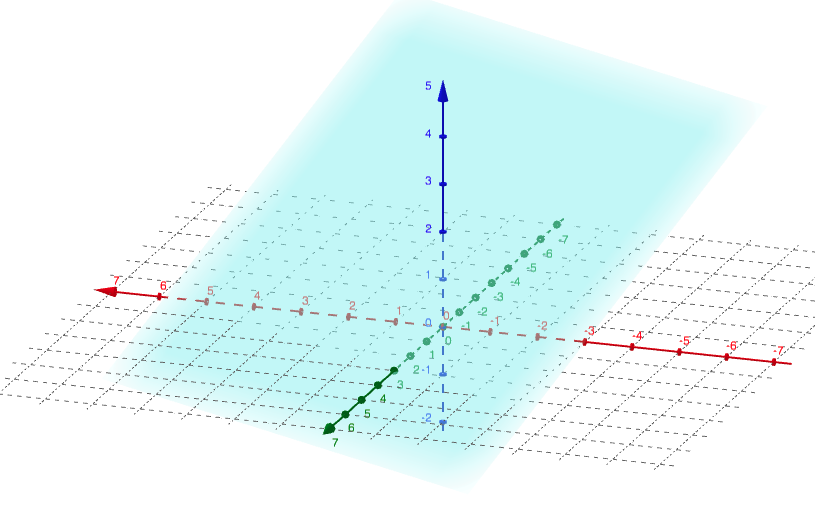
\includegraphics[scale = 0.5]{Pictures/plane3,1.png}

As we can see, the graph makes sense because:

\pagebreak
\textit{3,1,2: Graphicate the following:}

$$ z = 1-x = f(x,y) $$
\includegraphics*[scale=0.5]{plane3,1,2.png}
\pagebreak

\textit{3,1,3: Graphicate the following:}

$$ z = x^2 + y^2 $$

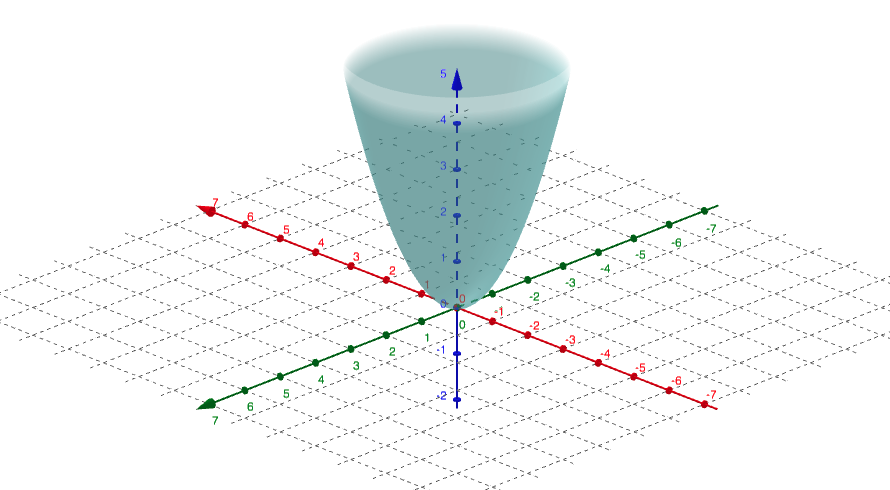
\includegraphics[scale = 0.5]{Pictures/plane3,1,3.png}
this is a three-dimensional parabola, also called more correctly as a circular paraboloid, comparable to it's two dimensional form, yet 
working on another dimension.

it can guarantee:

$$ \begin{cases}
    x = 0: z = y^2 \\
    y = 0: z = x^2
\end{cases}$$

and this equation can be deduced through this behavior. As:

$$ z = z_0 : x^2 + y^2 = z $$

there are level curves, which project the curve generated by such mathematical artifacts as a two dimensional
spherical object. Fields like topology or other 3-dimensional inclined math might regularly use it
when measuring space. In any case, a level curve could be illustrated as such:
\begin{center}
    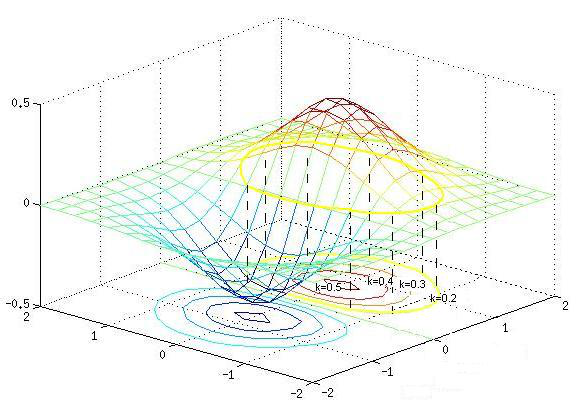
\includegraphics[]{Pictures/GraphCurves.png}    
    \textit{taken from: www.math.tamu.edu}
\end{center}

\section{Equations}

An equation, although similar to a function such as the ones studied so far,
can be distinguished by some particularities they present: 

$$ x^2 + y^2 + z^2 = 1$$

A few examples of objects described by equations are:

\subsection{Planes}

A plane is a 2-dimensional shape that can be expressed as:
\begin{equation}
    Ax + By + Cz = Ax_0 + By_0 + Cz_0
\end{equation}

There are different ways of getting the values regarded in this shape, as seen in 2.2.3 of these class notes, and we will mostly
do it by passing different geometrical expressions to a point and a vector normal to the plane, and replacing the vector 
on A,B,C, and the point in $ x_0, y_0, z_0 $

\paragraph{Example}

Find a plane normal to: $ \vec{n} = \begin{pmatrix}
    1 \\
    2 \\
    3 \\
\end{pmatrix} $
That passes through:
$ P = \begin{pmatrix}
    1 \\
    1 \\
    1 \\
\end{pmatrix} $

We replace fot this as following:

\begin{equation}
    1x + 2y + 3z = 1*1+2*1+3*1 \implies 1x + 2y + 3z = 6
\end{equation}

z = f(x,y) can also be a way to define a plane through a function, however, this is a bit 
limiting, as z is not free. However, tangent planes can be found in a fairly easy way

\subsection{Elipsoids}

An elipsoid is defined by the following equation:
\begin{equation}
    (\frac{x}{a})^2+(\frac{y}{b})^2+(\frac{z}{c})^2 = 1
\end{equation}


\subsection{Hyperboloid}

a Hyperboloid can be seen as:
\begin{equation}
    (\frac{x}{a})^2+(\frac{y}{b})^2 = (\frac{z}{c})^2 + 1
\end{equation}

\subsection{Cilinders}

The general formula of a cylinder is:

\begin{equation}
    (\frac{x}{a})^2+(\frac{y}{b})^2 = 1
\end{equation}

The level curves of this shape will never change when projected on a plane.

\subsection{Parabolic}

The general formula of a parabolic is:

\begin{equation}
    y = ax^2
\end{equation}

\subsection{Spheres}

\begin{equation}
    \begin{cases}
        x^2+y^2+z^2 = r^2 \\
        z \geq 0
    \end{cases}
\end{equation}

\subsection{Paraboloid}

The general formula of a paraboloid is:

\begin{equation}
    z = (\frac{x}{a})^2 + (\frac{y}{b})^2
\end{equation}

This shape has a variation, called a hyperbolic paraboloid:
\begin{equation}
    z = (\frac{x}{a})^2 - (\frac{y}{b})^2
\end{equation}

It will look like this when graphicated:
\begin{center}
    \includegraphics*[]{Pictures/hyperbolic_paraboloid.png}    
\end{center}

\section{Examples}

\paragraph{Calculate the tangent plane of $z e^z x y^2 = 0$ in the point $(\frac{\pi}{2},1,0)$}

\textit{Solution}
\begin{gather}
    z e^z x y^2 = 0 \\
    f(x,y) = \cos x \sin y e^z \\
    \begin{cases}
    \frac{\partial_F}{\partial_x} = - \sin x \cos y e^z  \\
    \frac{\partial_F}{\partial_y} = - \cos x \cos y e^z \\
    \frac{\partial_F}{\partial_z} =  \cos x \cos y e^z
    \end{cases} \\
    \frac{\partial_F}{\partial_x} = - \sin \frac{\pi}{2} \cos (1) e^0 = - \cos (1)\\
    \frac{\partial_F}{\partial_y} = - \cos \frac{\pi}{2} \sin 1 e^0 = 0 \\
    \frac{\partial_F}{\partial_z} = 0 \\
    - \cos(1) (x - \frac{\pi}{2}) + 0(y-1) + 0(z-0) = 0 \\
    - \cos (1) (x - \frac{\pi}{2}) = 0 \\
    x - \frac{\pi}{2} = 0\\
    x = \frac{\pi}{2}
\end{gather}


\chapter{Limits and continuity}
\subsection*{Sets and disks}
An open disk of radio 'r' and contourn $\vec{x}$ can be defined as


\begin{equation}
    \text{Let: }\vec{x}\exists\mathbb{R}^n , r > 0 \\ D_r = \{ \vec{x} \exists \mathbb{R}^n: ||\vec{x} - \vec{x_0} || < r \}
\end{equation}

and a disk that includes the internal values could be defined as 

\begin{equation}
    \text{Let: }\vec{x}\exists\mathbb{R}^n , r > 0 \\ D_r = \{ \vec{x} \exists \mathbb{R}^n: ||\vec{x} - \vec{x_0} || \le r \}
\end{equation}

Both of these are an important definition of what we'll call a \textbf{set}. 

let $$ \mu \subseteq \mathbb{R}^n $$ we can say that $\mu$ is an open set if  for any point $x_0 \exists \mu$
there exists a r>0 such as $$D_r(x_0) \subseteq \mu$$

Such sets have a mathematical structure called frontier points that can be defined as:
\paragraph*{Frontier point}
Let $ A \subseteq \mathbb{R}^n $; a point '$x \exists \mathbb{R}^n$' is a frontier point if any $ \vec{x} $
vecinity contains a point of A and at least a point outside of A

\paragraph*{Example}

Prove that '$A = (x,y)\exists\mathbb{R}^2: y > 0$' is an open set

Given that the open set can be inferred by a disk, we can affirm:

\begin{gather}
    \implies y>0 \implies r = \frac{y}{2} > 0 \\
    \text{If : }(a,b)\exists D_r(x,y)\\
    | b-y | \le \sqrt{(a-x)^2 + (b-y)^2} < r = \frac{y}{2} \\
    |b-y| < \frac{y}{2}\\
\end{gather}

\section{Limits}
A limit can be defined as

$ \lim_{x \to a} f(x) = L $

Where:

$ \forall \epsilon > 0 \exists \varrho > 0: | f(x) - L | < \epsilon $
for all X, such as 

$ 0 < |x-a| < \vartheta $

Or when said in words; "for every epsilon greater than zero that exists in a theta greater than zero, the function of value x minus L is lesser than epsilon for all X, such as the norm is greater than zero and smaller than theta".

For a limit to exist, we need three conditions to be met:

\begin{itemize}
    \item there is a left limit
    \item there is a right limit
    \item they're equal
\end{itemize}


\subsubsection{Multivariable limits}

a limit in a multi variable plane can be defined as: 

\begin{gather}
    \lim_{(x,y) \to (a,b)} = \vec{L}
\end{gather}

Meaning that we can force $ |f(x,y)-L|$ to be as near to zero as posible, making
(x,y) and (a,b) as close as possible without them actually ever touching each other.

Or, more formally;

\begin{gather}
    f: \mathbb{R}^n \to \mathbb{R}^m \\
    \text{Let: } f: A \subseteq \mathbb{R}^n \rightarrow \mathbb{R}^n \text{and :}\\
    \text{let $ \vec{x_0} \exists A $ or $ \vec{x_0} \exists \varTheta A $ }\\
    \lim_{x \to x_0} f(\vec{x}) = L \exists \vartheta \exists A \implies 0 < ||\vec{x} - \vec{x_0}|| < \vartheta, \implies ||f(\vec{x})-L||<\epsilon
\end{gather}

\subsection{Differentiation}

a function in a single variable can have every single point on a curve being approximated to
a line, called a tangent. This z = (x,y) line variable can be defined by partial derivatives, that
can be described as:
\begin{equation}
    z_x = \frac{D_z}{D_x} = \frac{D_f}{D_x} (x,y) = \lim_{h \to 0} = \frac{(x+h,y)-f(x,y)}{h} 
\end{equation}
\begin{equation}
    \frac{d_f}{d_y}(x,y) = \lim_{h \to 0} = \frac{(x,y+h)-f(x,y)}{h}
\end{equation}
Where 'h' is a real number that tends towards zero.

\paragraph*{Example: }
\textit{let: }
\begin{gather}
    f(x,y) = x^2-y^3 - 3x^4y
\end{gather}
\textit{then, differentiate the equation.}

\textbf{solution:}

\begin{gather}
    \frac{d_f}{d_x} = 2xy^3 - 12x^3y \\
    \frac{d_f}{d_y} = 3x^2y^2 - 3x^4
\end{gather}

When differentiating an equation on a specific variable, we take the other variables as constants.
In this example, we leave 'x' untouched when differentiating on 'y' and viceversa.

\subsection{Implicit differentiation}

We can think of an implicit derivative as the process of using partial derivatives to 
differentiate a single, more complex equation. 

\paragraph{Examples: }

\begin{itemize}
    \item a line that goes through $ \frac{y - y_0}{x - x_0} $

\end{itemize}

For three dimensions we might imagine instead of a line being the tangent, a 
plane providing the same definition and mathematical role as it, defined as:

\begin{gather}
    z = f(x, y_0) : z - z_0 = \frac{d_f}{d_x}(x, y_0)(x-x_0) \\
    z = f(x_0, y) : z - z_0 = \frac{d_f}{d_x}(x_0, y)(y-y_0)
\end{gather}

and with both this derivatives, we can define a plane as 

\begin{equation}
    z - z_0 = a(x-x_0) + b (y-y_0) \text{\textit{Where: }} \begin{cases}
        a = \frac{d_f}{d_y}f(x_0, y_0)\\
        b = \frac{d_f}{d_x}f(x_0,y_0)
    \end{cases}
\end{equation}

IF: $ x = x_0 = 0 $ and $ y = y_0$

We can approximate a three-dimensional differentiation as 

\begin{gather}
    d_z = fx(x_0, y_0)(x - x_0) + f_yfx(x_0, y_0)(y - y_0)\\
    f(x,y) \approx f(x_0, y_0) + d_z
\end{gather}

\textit{note: tangent planes are a very popular test/quiz problem, you should
learn how to find them for such ventures, if your professor ever mentions them
in class and ESPECIALLY if they try to solve one in front of the class.}

We can say that a function $ f: \mathbb{R}^2 \to \mathbb{R} $ is differentiable if:

\begin{equation}
    \Delta f = d_f + \epsilon_1 \Delta x +\epsilon_2 \Delta y 
\end{equation}

\noindent This deffinition is a bit hard to applicate, so we'll use the differentiation criteria for 
looking for appliability.

\textit{Appliability Criteria: }
We will say it is possible to differentiate a function if every partial derivative in $\frac{d_f}{d_{xj}}$
and if they're continuous in an open set 'D'.

\paragraph*{Example:}
\begin{gather}
    f(x,y) = \begin{cases}
        0 \implies (x, y) = (0,0) \\
        x^2 + y^2 \implies (x,y) \neq (0,0)
    \end{cases} \\
    \frac{df}{dx} (0,0)= \lim_{h \to 0}  \frac{f(h, 0) - f(0,0)}{h} = \lim_{h \to 0}  \frac{0 - 0}{h} = 0 \\
    \text{BUT THEN, that means a partial derivative for (0,0) does not exist,}\\ \text{ therefore this is not a continuous function.} \\
    \lim_{(x,y) \to (0,0)}  \frac{xy}{x^2+y^2} NE
\end{gather}

\subsection{Examples}
\begin{itemize}
    \item Solve:

\begin{equation}
    \lim_{(x,y) \to (0,0)}  \frac{\cos - 1 - \frac{x^2}{2}}{x^4+y^4}
\end{equation}

This limit \textbf{DOES NOT EXIST}:

because going by paths we can assume:

$$<x=0>$$

Would imply:
\begin{gather}
    \lim_{y \to 0} \frac{\cos 0 - 1 - \frac{0^2}{2}}{0^4 + y^4} \\
    \lim_{y \to 0} \frac{0}{y^4} = \lim_{y \to 0} 0 = 0
\end{gather}

$$<y=0>$$

Would imply:
\begin{gather}
    \lim_{x \to 0} \frac{\cos x - 1 - \frac{x^2}{2}}{x^4} \implies \frac{0}{0} \\
    \text{<l'Hopital because of indetermination>}\\
    \lim_{x \to 0} \frac{- \sin x - x}{4x^3} \\
    \text{<l'Hopital because of indetermination... again.>} \\
    \lim_{x \to 0} \frac{- \cos x - 1}{12x^2} \\
    \dots
\end{gather}

...and it will never stop differentiating until a $\mathbb{R}$ value is divided by 0, which
isn't possible without adding multiple things to our framework of reference, maybe imaginary numbers or
something.


we can graphicate such a function as:

\begin{center}
    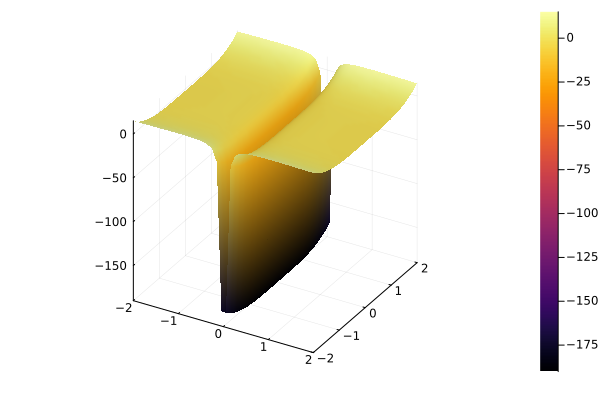
\includegraphics[scale=0.5]{Pictures/4131.png}    
\end{center}

Would imply:
\end{itemize}
\section{Continual Functions}

A function can be defined as continual if a limit can be described as:

\begin{itemize}
    \item $$\lim_{\vec{x} \to \vec{x}_0}f(x) = f(X_0) = f(\lim_{\vec{x} \to \vec{x_0}} \vec{x})$$
\end{itemize}

This would mean that a limit is replaceable by a function where the limit of $\vec{x}$ 
is described according to the mathematical rules that define a function. 
if a function is continual and has $\frac{D_{fi}}{D_{xj}}$ then it's differentiable


\section{Tangent Planes}
 We tangentially touched this topic on implicit differentiation, however, to define more 
 formally a tangent plane,
 
 Let:

 \begin{gather}
    f: A \subseteq \mathbb{R}^2 \to R \\
    \vec{\Delta} f (x,y) = < \underbrace{\frac{D_f}{D_x} (x,y)}_\text{Partial Derivative of X}, \underbrace{\frac{D_f}{D_y} (x,y)}_\text{Partial Derivative of y}> \\
    f(x_0, y_0) + D(f(\vec{x})) (\vec{x}-\vec{x_0})
 \end{gather}


\section{Derivative Properties}
\subsection{Constant multiple rule}
$$ \frac{\delta}{\delta_x}(c f(x,y)) = c \frac{\delta}{\delta_x}(f(x,y)) $$
\subsection{Sum rule}
$$\frac{\delta}{\delta_x}(f(x,y) + g(x,y)) = \frac{\delta_f}{\delta_x} f(x,y) + \frac{\delta_g}{\delta_x} g(x,y)$$
\subsection{Product rule}
$$\frac{\delta}{\delta_x}(f(x,y) \centerdot g(x,y)) = \frac{\delta_f}{\delta_x} f(x,y) g(x,y) + \frac{\delta_g}{\delta_x} g(x,y) f(x,y)$$
\subsection{Divisor rule}
$$\frac{\delta}{\delta_x}(\frac{f}{g})(x,y) = \frac{\frac{\delta_f}{\delta_x} f(x,y) g(x,y) - \frac{\delta_g}{\delta_x} g(x,y) f(x,y)}{[g(x,y)]^2}$$
\subsection{Chain Rule}

\subsubsection{One variable}
If $\vec{u}(x)$ and $\vec{x}(t)$ are differentiable, then: 

$$\frac{\delta_u}{\delta_t} = \frac{d_y}{d_x} \frac{d_x}{d_t} = u'(x|t|) + x'(t)$$

\subsubsection{Two variables}

Given  $\vec{w}(x,y)$, $\vec{u}(x,y)$ and $\vec{v}(x,y)$, then $w(u(x,y), v(x,y))$ is differentable.

so, therefore:

\begin{gather}
    y = 
    \begin{cases}
        \frac{\delta w}{\delta x} = \frac{\delta w}{\delta u} \frac{\delta u}{\delta x} + \frac{\delta w}{\delta v} \frac{\delta v}{\delta x} \\
        \frac{\delta w}{\delta y} = \frac{\delta w}{\delta u} \frac{\delta u}{\delta y} + \frac{\delta w}{\delta v} \frac{\delta v}{\delta y} 
    \end{cases}
\end{gather}


In general, we can define this rule as 
\begin{equation}
    D(f o g) = Df(g(\vec{x_0})) Dg(\vec{x_0})
\end{equation}

\section{Gradients and directional derivatives.}

assume a 3D plane as such:

\begin{center}
    \includegraphics*[scale = 0.5]{plane.png}
\end{center}

Def: a directional derivative is given by:

\begin{equation}
    D_{\vec{u}}f(x_0,y_0) = \frac{d}{dt} f(x_0 + t u_1, y_0 + t u_2) ; t = 0
\end{equation}

And we say that if a derivative exists, then $||\vec{u}|| = 1$;
f depends on x and y, and x and y both depend on t, this can be seen mathematically as:

\begin{equation}
    \frac{df}{dx} f(x_0 + t u_1, y_0 + t u_2) \underbrace{U_1}_{\frac{dx}{dt}} + \frac{df}{dy}(x_0 + t u_1, y_0 + t u_2) \underbrace{U_2}_{\frac{dy}{dt}}
\end{equation}

from this we can observe
\begin{equation}
    D_{\vec{u}}\ f(x_0, y_0) = \vec{\Delta} f(x_0, y_0) \centerdot \vec{u} = ||\vec{\Delta} f(x_0,y_0)|| \centerdot ||\vec{u}|| \centerdot \cos \theta\\
\end{equation}

So, given this set of conditions:

\begin{gather}
    \begin{cases}
        D_{\vec{u}} f(x_0, y_0) \text{  is maximal if $ \theta $ is 0} \\
        D_{\vec{u}} f(x_0, y_0) \text{  is minimal if $ \theta $ is $\pi$}
    \end{cases}
\end{gather}

We can infer then, regarding our direction:

\begin{equation}
    \vec{u} = \frac{\vec{\Delta} f(x_0, y_0)}{||\vec{\Delta}f(x_0,y_0)||}
\end{equation}

will make the function grow faster, and:

\begin{equation}
    \vec{u} = - \frac{\vec{\Delta} f(x_0, y_0)}{||\vec{\Delta}f(x_0,y_0)||}
\end{equation}

will make it decrease faster.
 

\subsection{implicit equations}

An implicit surface equation given by $F(x,y,z) = C$ we can define, as a curve:

\begin{gather}
    \vec{r}t = <x(t),y(t),z(t)> \\
    \vec{r}t' = <x'(t),y'(t),z'(t)> 
\end{gather}

And from there we can assume that this curve is a part of S if:

\begin{gather}
    F(x(t), y(y), z(t)) = C ; \forall t
\end{gather}

Given this, F depends on x,y, and z and those three variables depend on t, allowing us
to affirm:

\begin{gather}
    F_x \frac{dx}{dt} + F_y \frac{dy}{dt} + F_z \frac{dz}{dt} \\
    \vec{\Delta} f \centerdot \vec{r}t' = 0
\end{gather}

geometrically this means the gradient is perpendicular to the tangent and therefore, the tangent plane.
to S in $(x_0,y_0,z_0)$, which can be expressed vectorially (and therefore, more usefully) as:

\begin{equation}
    \vec{\Delta}F(x_0,y_0,z_0) \centerdot \begin{pmatrix}
        x - x_0 \\ 
        y - y_0 \\ 
        z - z_0
    \end{pmatrix} = 0
\end{equation}

The line normal to S in $(x_0,y_0,z_0)$ can be defined as:

\begin{equation}
    \vec{n}(t) = \vec{x_0} + t\vec{\Delta} F(x_0,y_0,z_0)
\end{equation}

\section{Iterated Partial derivatives:}

\paragraph*{addendum}

Remember:
\begin{itemize}
    \item $f \exists C^o$ means a function is continuous
    \item $f \exists C^1$ means f' is continuous
    \item $f \exists C^k$ means the k derivative is continuous
\end{itemize}

\subsection{Iterated derivatives}
let:

\begin{equation}
    f(x,y) = x^2 y^3 - 3x^4 y
 \end{equation}

then:

\begin{gather}
    f_x(x,y) = 2xy^3 - 12x^3 y \\
    f_y(x,y) = 3x^2 y^2 - 3x^4 \\
    f_{xx} = 2y^3 - 36x^2y \\
    f_{xy} = 6xy^2 - 12x^3 \\
    f_{yx} = 6xy^2 - 12x^3 \\
    f_(yy) = 6x^2y
\end{gather}

As we can see, equations 4,51 and 4,52 are equivalent, this is because when we do
such chained differentiations, we can guarantee:

\begin{equation}
    \frac{\partial}{\partial y} (\frac{\partial f }{\partial x}) = \frac{\partial^2 f}{\partial y \partial x}
\end{equation}

\subsection{Clairaut's Theorem}

If $ f(xy), f(yx) $ are continuous, then $f_{xy} = f_{yx}$ 

\subsubsection*{Proof}

Okay, this might get a bit technical, but here we go:

As written by Kiril Datchev from Purdue\cite[]{} (give his stuff a read, it's pretty cool), we can take as a given:

By definition:
\begin{itemize}
    \item \begin{equation}
        \partial_x \partial_y f(a,b) = \lim_{h \to 0} \frac{\partial_y f(a + h, b) - \partial_y f(a,b)}{h}
    \end{equation}
\end{itemize}

So from this, we can deduce:
\begin{gather}
    \\
\end{gather}

\section{Examples}

\paragraph*{Find the gradient in P=(0,3) if $f(x,y)=2ye^{xy}+ y \cos x$} 
We can use what we know of partial derivatives to affirm:
\begin{gather}
    \vec{\Delta}f(x,y) = <2y^2 e^{xy} - y \sin x ; 2e^{xy}+2xe^{xy} + \cos x>;\\
    \text{<replace for P>};\\
    \vec{\Delta}f(0,3) = <2*3^2 e^{0*3} - 3 \sin 0 \ ; \ 2e^{0*3} + 2* 0 *e^{0*3} + \cos (0)>;\\
    \vec{\Delta}f(0,3) = <18,3>
\end{gather}

\paragraph*{Find the derivative in $f(x,y) = \frac{x}{y}$ in the point
(6,-2) and the direction of $\vec{v} = <1,3>$} 

This can be said as:
\begin{gather}
    \vec{\Delta}(x,y) = <\frac{1}{y},-\frac{x}{y^2}>;\\
    \vec{\Delta}(6,-2) = <- \frac{1}{2},-\frac{3}{2}>
\end{gather}

Given this initial state, we can then use the following declarations on this problem:

\begin{gather}
    ||\vec{v}|| = \sqrt{10};\\
    \vec{u} = \frac{\vec{v}}{||\vec{v}||} = \frac{1}{||\vec{v}||} \vec{v}
\end{gather}

And therefore, conclude:

\begin{equation}
    D_{\vec{u}}f(6,-2) = \frac{1}{\sqrt{10}} (\frac{1}{2} - \frac{9}{2}) = \frac{4}{\sqrt{10}} = -\sqrt{\frac{8}{5}}
\end{equation}

\paragraph*{Find the change rate in $h(x,y,z) = \cos(xy)+e^{yz}+\ln(xz)$ in the point
(1, 0, 0.5) moving towards $P_1 = (2,2,\frac{5}{2})$} 

Much as in our first example, we can use partial derivatives to get a delta for this problem.
The change rate of a function \textbf{Is the same as a derivative, for a derivative is interested in
how much a function changes}; we shall then affirm:

\begin{equation}
    \vec{\Delta}h(x,y,z) = <-\delta \sin(x,y) + \frac{1}{x}, - x \sin y +ze^{yz}, ye^{yz} + \frac{1}{z} >
\end{equation}

\paragraph*{Find the tangent plane and normal line of:}
$x^2 + y^2 = -4+2xy + x - 3y + z^2$ in $P=(1,2,\sqrt{10})$

We can reweite this as: 

\begin{gather}
    F(x,y,z) = -4 \\
    \vec{\Delta} F (x,y,z) = <2x-2y-1; 2y - 2x + 3, -2z > \\
    \vec{\Delta} F(1,2,\sqrt{10}) = <-3,5,-2 \sqrt{10}>
\end{gather}

From here, we can define the plane as:
\begin{gather}
    -3(x-1) + 5(y-2) - 2 \sqrt{10}(z-\sqrt{10}) = 0 \\
    -3x + 5y - 2\sqrt{10} z = -13 \\
    3x - 5y + 2\sqrt{10} z = 13
\end{gather}

And the line can be defined therefore as:
\begin{equation}
    \vec{n}(t) = \begin{pmatrix}
        1 \\
        2\\
        \sqrt{10}
    \end{pmatrix} + t \begin{pmatrix}
        -3 \\
        5 \\
        -2 \sqrt{10}
    \end{pmatrix}
\end{equation}

Just as a curiosity, we can write the curve as this:
\begin{center}
    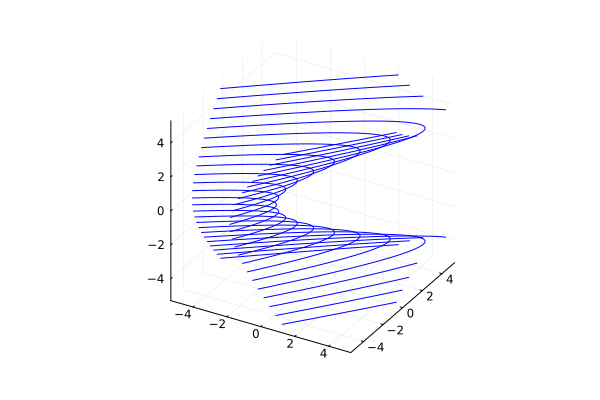
\includegraphics[scale=0.5]{Pictures/473.png}
\end{center}

\section{important expressions}
\begin{itemize}
    \item Tangent Planes:
    \begin{equation}
        \frac{\delta F}{\delta x}(x_0,y_0,z_0)(x-x_0) + \frac{\delta F}{\delta y}(x_0,y_0,z_0)(y-y_0) + \frac{\delta F}{\delta z}(x_0,y_0,z_0)(z-z_0) = 0 
    \end{equation}
    \item Directional Derivative:
    \begin{equation}
        \frac{d}{dt}f(x_0+tu,y_0+tu_z) | 0
    \end{equation}
\end{itemize}

\chapterimage{Heading4.jpg} % Chapter heading image

\chapter{Superior order derivatives}

\section{Taylor's Theorem}
let

$$ f: \mathbb{R} \to \mathbb{R} $$

Then:
\begin{equation}
    F(x) = F(a) + F'(a) (x-a) + \frac{F''(a)}{\alpha !} (x-a)^2 + \dots + \frac{F^{(k)}(x-a)^k}{k!} (x-a)^k + error    
\end{equation}

this can also be written as:
\begin{equation}
    \Delta F(t_0) = F(t_0+\Delta t) - F(t_0)
\end{equation}

Generally, we can assume that given a theorem from $\mathbb{R}^n \to \mathbb{R}^n$

\begin{gather}
    \vec{x_0} = \begin{pmatrix}
        x_1 \\
        . \\
        . \\
        . \\
        x_n
    \end{pmatrix} ,
    \vec{h} = \begin{pmatrix}
        h_1 \\
        . \\
        . \\
        . \\
        h_n
    \end{pmatrix} \text{then:} \\
    f(\vec{x_0}+ \vec{h}) = f(\vec{x}_0) + \sum_{1}^{n} \frac{\partial f}{\partial x_i}(\vec{x_0}) + \frac{1}{2!} \sum_{i,j = 1}^{n} h_i h_j \frac{\partial^2 f}{\partial x_i \partial x_j} \vec{x_0} +  
    \frac{1}{3!} \sum_{i,j,k = 1}^{n} h_i h_j h_k \frac{\partial^3 f}{\partial x_i \partial x_j \partial x_k} \vec{x_0} + \dots 
\end{gather}

...That being said, we can mostly just stay with two. Triple derivatives are sure as hell weird. 

\section{Function extremes with real values.}

Given a set 'D' that is bound if we can find a value R > 0 such as:
$$ D \subseteq x^2 + y^2 \leq R^2 $$
and:
$$ D \subseteq \mathbb{R}^2 \to \mathbb{R} $$

We can express this as:
\begin{gather}
    f: D \subseteq \mathbb{R}^2 \to \mathbb{R} \\
    p \exists D \ is: \ \begin{cases}
        \max \ if \ f(p) \geq f(x) \forall x \exists D \\
        \min \ if \ f(p) \leq f(x)   
    \end{cases}
\end{gather}

And we can also localize this to a specific region of the set, as a local
minimum or maximum, think of it as p being a subset of a set, and then write it
in the same way as you write above:


\paragraph{Theorem: }

'f' has a local maximum or a minimum in $(x_0, y_0)$ , 
if an interior point of D and the partial derivatives of 'f' exist in
$ (x_0, y_0) $ , then:

\begin{gather}
    f_x = (x_0, y_0) = 0 \wedge f_y(x_0, y_0) = 0
\end{gather}

\subsection{Critical Points}

p is a critical point of an f function if all partial derivatives are zero in such a point. 

given a continuous function $f: D \to \mathbb{R} $
that's closed and bound, then f will achieve its 
minimum and maximum values.

\paragraph{Example}
\begin{gather}
    f(x,y) = x^2 + y^2 = \begin{cases}
        f_x = 2x = 0 \\
        f_y = 2y = 0
    \end{cases} \min(0,0)
\end{gather}

We can see similar behavior in a hyperbolic paraboloid, but here, it wont be an absolute minimum for both points.

\paragraph{Example}
\begin{gather}
    f(x,y) = x^2 - y^2 = \begin{cases}
        f_x = -2x = 0 \\
        f_y = -2y = 0
    \end{cases}
\end{gather}

Every critical point is a candidate to be an absolute maximum or minimum, but won't nescessarily be. 
in any case, partial derivatives are a good tool for finding them through the critical points of a function.

If f has continuous second-order continuous derivatives, then:

\begin{equation}
    \vec{D}^2_{\vec{u}} f(x_0,y_0) = \vec{D}_{\vec{u}} \vec{D}_{\vec{u}} f(x_0,y_0)\\
\end{equation}

Is a directional derivative of (x,y) in u , we can calculate it as:

\begin{gather}
    D_{\vec{u}}f(x,y) =\vec{\nabla} f \centerdot \vec{u} = <fx, fy> \centerdot <h,k> \\
    \vec{\nabla}(h f_x+ k f_y) \centerdot \vec{u} = <h f_{xx} + k f_{yx}, h f_{xy} + k f_{yy}>
\end{gather}

By developing this further, we'll arrive to a discriminant matrix of the sort:

\begin{equation}
    \begin{pmatrix}
        f_{xx} & f_{xy} \\
        f_{yx} & f_{yy}
    \end{pmatrix} = det
\end{equation}

from whatever this gives us, we can say:

\begin{equation}
    D = det \implies \\
    \begin{cases}
    \text{if: } D > 0 \wedge  f_{xx} > 0 \implies (x_0 , y_0) = \min \text{ local} \\
    \text{if: } D > 0 \wedge  f_{xx} < 0 \implies (x_0 , y_0) = \max \text{ local} \\            
    
    \end{cases}
\end{equation}

\section{Restricted extremes and Lagrange multiplicators}

\begin{center}
    \includegraphics*[]{Pictures/lagrange.jpg}
\end{center}

Given a curve 'C' in the plane x,y in the plane: g(x,y) = k,
given that g has $\partial '$ and $\vec{\Delta} g \neq 0$,
finding minimums and maximums of f(x,y) alongside 'C.
f has continuous $\partial '$. 

If we assume f to have a maximum or minimum in $(x_0, y_0)$, then:
\begin{gather}
    D_{\vec{T}}f(x_0,y_0) = 0 \\
    \underbrace{\vec{\Delta}f(x_0,y_0)}_{\exists \mathbb{R}^2} \centerdot \underbrace{\vec{I}}_{\exists \mathbb{R}} = 0
\end{gather}

If we assume f(x,y,z) having an extreme point $(x_0,y_0,z_0)$ on a surface S:
$g(x,y,z) = k$ then for a plane P:

\begin{gather}
    D_{\vec{u}}f(x_0,y_0,z_0) = 0 \forall \vec{u} \exists P \\
    \vec{\triangledown} f(x_0,y_0,z_0) = 0 \forall \vec{u}\\
\end{gather}

Imagine the following function:

$$ z =  x^2 + xy + y^2 $$

with every point being part of $\mathbb{R}^2$, if we were to find local minimums and maximums,
therefore:

\begin{gather}
    f(x,y) =  x^2 + xy + y^2 \\
    \partial_x = 2x + y\\
    \partial_y = x + 2y\\
    \begin{cases}
        2x + y = 0\\
        x + 2y = 0
    \end{cases}
    \implies \begin{pmatrix}
        2 & 1 \|\ 0\\
        1 & 2 \|\ 0\\
    \end{pmatrix}\\
    x=0 ; y=0\\
    (0,0)
\end{gather}

from there, we can imagine a Hessian matrix.

\section{Implicit function theorem}

Let a function 'F(x,y) = 0' that is the implicit equation of a curve in xy;
then:

\paragraph*{Example}
\begin{gather}
    \frac{x^2}{a^2} + \frac{y^2}{b^2} - 1 = 0 \\
    y = \pm \sqrt{(1-\frac{x^2}{a^2})b^2} = \pm \sqrt{\frac{b^2}{a^2}(a^2 - x^2)}; x \exists [-a, a]
\end{gather}

This is an example of a situation where fiven F(x,y)=0 and $ (x_0, y_0) $, expressed together
as $F(x_0,y_0)=0$ we would like to know if we gan obtain

\subsection{Theorem 1}
Let:

\begin{itemize}
    \item a F(x,y) defined and continuous in a rectangle centered on our point $(x_0, y_0)$; then
    $ D = [x_0 - \triangle, x_0 + \triangle; y_0 - \triangle, y_0 + \triangle] $
    \item $F(x_0, y_0) = 0$
    \item $y \rightarrow F(x,y)$ increases (or reduces) in a strictly monotonous fashion.
\end{itemize}

Then:

\begin{itemize}
    \item in a vecinity of the point, (*) can determine as a function of $x: y = f(x)$
    \item $f(x_0) = y_0$
    \item f is continuous
\end{itemize}

\subsection{Theorem 2}

We'll assume, besides that we assumed on our first theorem:
\begin{itemize}
    \item $F_y = (x_0,y_0) \neq 0$
    \item $\partial_x, \partial_y$ exist and are continuous.
\end{itemize}

Then, including what we concluded on the first iteration, we can conclude that:
\begin{itemize}
    \item in a vecinity of the point, (*) can determine as a function of $x: y = f(x)$
    \item $f(x_0) = y_0$
    \item f is continuous
    \item f'() exists and is continuous
\end{itemize}

let's remember a function is differentiable when:

\begin{gather}
    F_x (x,y) \Delta x + F_y (x,y) \Delta y + \epsilon_1 \Delta x + \epsilon_2 \Delta y, \epsilon_1, \epsilon_2 \rightarrow 0 \\
    = \Delta x (F_x(x,y) + \epsilon_1) + \Delta y (F_y (x,y)+ \epsilon_2) \\
    \frac{\Delta y}{\Delta x} = - \frac{F_x + \epsilon_1}{F_y = \epsilon_2}, \lim_{\Delta x \to 0} \frac{\Delta y}{\Delta x} = - \frac{F_x(x,y)}{F_y(x,y) \neq 0}\\
    f'(x)
\end{gather}

\subsection{Theorem 3}

We assume:
\begin{itemize}
    \item $F(x_1,\dots,x_n, y)$ is defined and continuous over $D = [\dots]$
    \item $f(x_1^0,\dots,x_n^0,y_0) = 0$ \\
    \item $f_y \neq 0$
    \item $f_{x1}, \dots, f_{xn}, f_y$ exist and are continuous
\end{itemize}

then:

\begin{itemize}
    \item in a vecinity $(x_1^0, \dots, x_n^0, y_0),(**)$ determines as a function
\end{itemize}

\subsection{General Theorem}

In general, we'll say that $F_1(x_1 \dots, x_n, y_1, \dots, y_n) = 0 = (***)$

then $\underbrace{(***)}_{determines} y_1, \dots, y_n$ as functions of  $x_1, \dots, x_n$ 
if for every $(x_1, \dots, x_n) \exists (a,b, \dots; \dots) = z$ the system has a single solution
$y_1, \dots, y_n$

Instead of $F_y (x_0, y_0) \neq 0$ we can say that a Jacobian can be determined as a Hessian of the type:

\begin{gather}
    J = \frac{D(F_1, \dots, F_n)}{D(y_1, \dots, y_n} = \begin{vmatrix}
        \frac{\partial F_1}{\partial y_1} & \dots & \frac{\partial F_1}{\partial y_n} \\
        \dots & \dots & \dots \\
        \frac{\partial F_n}{y_1} & \dots & \frac{\partial F_n}{y_n} 
    \end{vmatrix}
\end{gather}

Put under the logic of the previous statements, we would say:

\begin{itemize}
    \item $F_i$ is defined and continuous
    \item The point $(x_1^0, \dots , y_n^0;y_1^0, \dots , y_n^0)$ satisfies (***)
    \item $J(x_1^0, \ dots, y_n^0)\neq 0$ 
    \item $\partial '$ of $F_i$ are continuous in all variables
\end{itemize}

Then:

\begin{itemize}
    \item in a  $(x_1^0, \dots , y_n^0;y_1^0, \dots , y_n^0)$ vecinity it can be determined by (***)
    \item $f_j (x_1^0, \dots, x_n^0) = y_j^0$
    \item $f_j$ is continuous
    \item Partial derivatives of $f_j$ are continuous
\end{itemize}

\subsubsection*{Demonstration}
\begin{gather}
    m = 1 \ complies \ Theorem \ 3; \\
    \text{Theorem 3} m - 1 \implies \text{Theorem 3} m \\
    J(X_1^0, \dots y_1^0) \neq 0\\
    <induct \ \frac{\partial F_m}{\partial y_m}(x_1^0 \dots x_n^0) \neq 0 > \\
    <Theorem \ 3 = T_3>\\
    T_3 \implies F_m(x_1, \dots y_m) = 0; D^* \subseteq D\\
    y_m = f(n)(x,y)\\
    y_m = \phi (x_1 \dots x_n, y_1 \dots y_n)\\
    \implies F_m(x_1 \dots y_{m-1};\phi (x_1 \dots x_n, y_1 \dots y_n)) = 0, \\
    <\phi \ continuous \ ; \partial ' \ exist>\\
    J* = \frac{d(\phi_1, \dots \phi_m-1)}{d(y_1, \dots, y_{m-1})} = \begin{vmatrix}
        \frac{\partial \phi_1}{\partial y_0} & \dots & \frac{\partial \phi_1}{\partial y_{m-1}}\\
        \dots & \dots & \dots \\
        \frac{\partial \phi_1}{\partial y_{m-1}} & \dots & \frac{\partial \phi_{m-1}}{\partial y_{m-1}}
    \end{vmatrix}\\
    <Chain \ Rule>\\
    F_m(x_1, \dots, y_m-1, \phi (x_1, \dots, y_m-1)) = 0\\
    J = J^* \centerdot \frac{\partial F_m}{\partial y_m} \neq 0 \implies J \exists T_3
\end{gather}


\section{Examples}

\paragraph*{Given 3 non-negative numbers with a 120 overall sum, find the maximal value of x,y,z}
\begin{gather}
    x+y+z=120 \implies z = 120-x-y \\
    f(x,y) = xy(120-x-y)\\
    \{ x,y | x,y \exists \mathbb{R}^2 \geq 0; x \leq 120 - y; y \leq x - 120 \} \\
    \text{<Implies y = -x + 120 >}
\end{gather}

we can graph it as:

\begin{center}
    \includegraphics*[scale=0.5]{line.png}
\end{center}

from this we can say, by calculating the area:

\begin{equation}
    f(x,y) = 120xy -x^2y - xy^2
\end{equation}

And now we differentiate:

\begin{gather}
    f_x = 120y -2xy - y^2 \\
    f_y = 120x - 2xy -y^2 \\
    \text{<Minimals>} \\
    120 - 2x - y = 0 \implies x = 0 \vee y = 0 \
\end{gather}

and from linear algebra, we can do:

\begin{gather}
    \begin{pmatrix}
        -2 && -1 | -120 \\
        -1 && -2 | -120
    \end{pmatrix} 
\end{gather}

after solving this we can say:

\begin{gather}
    x = 40 \implies y = 40 \implies z = 40 \\
    f(40,40,40) = (40^3)
\end{gather}


%\paragraph*{find the absolute maximum and minimum of $f(x,y) = x^2+2xy+3y^$ in a closed triangle with vertices in $(-1,1),(2,1),(-1,2)$}

\paragraph{Find critical points of $z = x^2 + y^2 + 3xy$}

\begin{gather}
    \frac{\partial_z}{\partial_x} = 2x + 3y = 0 \\
    \frac{\partial_z}{\partial_y} = 2y + 3x = 0 \\
    \begin{cases}
        2x + 3y = 0 \\
        2y + 3x = 0
    \end{cases} \implies
    y = - \frac{2x}{3} \\
    2(- \frac{2x}{3}) + 3x = 0 \\
    - \frac{4}{3}x + 3x = 0 \\
    \frac{5}{3} x = 0 \\
    x = 0 \\
    y = 0 \\
    \text{\textit{(0,0) is the only critical point}}
\end{gather}

Now we might imagine:

$$D(\triangledown f) = \underbrace{H}_{\text{Hessian}} f(x,y) = 
\begin{pmatrix}
    \frac{\partial^2 f}{\partial x^2} & \frac{\partial^2 f}{\partial y \partial x} \\
    \frac{\partial^2 f}{\partial x \partial y} & \frac{\partial^2 f}{\partial y^2} 
\end{pmatrix}$$

And from that:

\begin{gather}
    \frac{\partial^2 f}{\partial x^2} = 2 \\
    \frac{\partial^2 f}{\partial x \partial y} = 3 \\
    \frac{\partial^2 f}{\partial y \partial x} = 3 \\
    \frac{\partial^2 f}{\partial y^2} = 2 \\
    \implies H = \begin{pmatrix}
        2 & 3 \\
        3 & 2
    \end{pmatrix} \\
    \Delta = det \ Hf (0,0) \\
    \Delta = -5 \\ \text{(Inflection point)}
\end{gather}

\paragraph{Find the absolute maximum and minimums of $f(x,y) = x^2+2xy+3y^2$
in a closed triangle with vertices in $(-1,1),(2,1),(-1,2)$}

\begin{gather}
    f_x = 2x+ 2y = 0 \\
    f_y = 2x + 6y = 0 \\
    <therefore> \\
    y = 1 \\
    0 \centerdot x - 4y +0 \implies y = 0; x = 0; f(0,0)=0 \\
    y = 1; f(x,1) = x^2+2x+3 \\
    x = -1\\
    g'(x) = 2x + 2 = 0 \implies x = -1 \implies f(-1,1) = 1-2+3 = 2\\
    g(y) = f(-1,y) = 1 - 2y + 3y^2\\
    g'(y) = 6y-2 + 0 \implies y = \frac{1}{3} \implies (-1, \frac{1}{3}), f(-1, \frac{1}{3}) = \frac{2}{3} \\
    y = x-1 \\
\end{gather}

\paragraph{Find the points over the surface $xyz = 8$
that are the closest to the origin (0,0,0)}
\begin{center}
%    \includegraphics*[scale=0.5]{xyz8.png}
    \textit{pictured: the surface to be analyzed}
\end{center}

\begin{gather}
    f(x,y) = \sqrt{x^2+y^2+\frac{6y}{x^2 y^2}} \\
    g(x,y) = x^2 + y^2 + \frac{6y}{x^2 y^2} \\
    \begin{cases}
        g_x = 2x - \frac{128}{x^3 y^2} \\
        g_y = 2y - \frac{128}{x^2 y^3}             
    \end{cases} \implies 2x^4 y^4 = 128 < = > x^4 = \frac{64}{y^2} <=> x^2 = \pm \frac{8}{y} \\
    <Case \ 1:> \ x^2 = \frac{8}{y}\\
    2y^4 x^2 = 128 \implies 2y^4 \frac{8}{y} \implies y^3 = 8 \implies y = 2 \implies x^2 = 4 \implies x \pm 2 \implies (2,2) \wedge (-2,2)\\
    <Case \ 2:> \ x^2 = - \frac{8}{y}\\
    \dots y^3 = -8 \implies y = -2 \implies x^2 = 4 \implies x \pm 2 \implies (2,-2) \wedge (-2,-2)\\
    f(\pm 2, \pm 2) = \sqrt{12}
\end{gather}

The closer points to the origin are (2,2,2), (-2,2,-2), (2,-2,-2), (-2,-2,2)

\paragraph{Find the extremes of $f(x,y) = xy$ alongside the elipse
$\underbrace{4x^2+y^2=4}_{g(x,y)}$}
Note: extreme values are different from 0, and xy is different from 0

\begin{gather}
    \vec{ \triangledown } f(x,y) = \lambda \vec{\triangledown} g(x,y)\\
    <x,y> = \lambda <8x,2y> <=> \begin{cases}
        y = \lambda 8x: I \\
        x = \lambda 2y: II \\
        4x^2 + y^2 = 4: III
    \end{cases} \\
    \frac{I}{II}: \frac{y}{x} = \frac{4x}{y} <=> y^2 = 4x^2 \\
    4x^2 + 4x^2 = 4 \\
    8x^2 = 4 \\
    x^2 = \frac{1}{2} \\
    x \pm \frac{1}{\sqrt{2}} \\
    y^2 = 2, y \pm \sqrt{2}
\end{gather}

\paragraph{Find the volume of a rectangular box defined by three planes and a vertex in (0,0,0),
under $3x + 2y + z = 6$}

\begin{gather}
    f(x,y,z) = xyz \\
    \vec{\triangledown}f(x,y,z) = \lambda \vec{\triangledown} g (x,y,z) \\
    <yz,xz,xy> = \lambda <3,2,1> \\
    \begin{cases}
        yz = 3 \lambda \\
        xz + 2 \lambda \\
        xy = \lambda \\
        3x + 2y + z = 6
    \end{cases}\\
    \frac{I}{II} <=> \frac{y}{x} = \frac{3}{2} <=> 2y = 3x \\
    \frac{II}{III} <=> \frac{7}{y} = 2 <=> z = 2y\\
    3x+3x+3x=6\\
    9x=6 \implies x = \frac{2}{3} \implies y = 1 \\
    \implies z = 2
\end{gather}

\paragraph*{Calculate critical points of the following function: $f(x,y) = x^2 y - xy^2 - x+y$}

\begin{gather}
    \Delta f(x,y) = (\overbrace{2xy-y^2-1}^{\frac{\partial f}{\partial x}}, \overbrace{x^2-2xy+1}^{\frac{\partial f}{\partial y}})\\
    \Delta f(x,y) = (0,0) <=> f_x = 0, f_y = 0\\
    \begin{cases}
        2xy-y^2-1=0\\
        x^2-2xy+1=0
    \end{cases}\\
    2xy-y^2-1=0\\
    2xy = y^2 + 1\\
    x^2 - (y^2 + 1) + 1 = 0 \\
    x^2 = y^2 \\
    |x| = |y|\\
    y = \pm x \implies
    \begin{cases}
        C1 = y = x \\
        C2 = y = -x
    \end{cases}\\
    <C1>\\
    y = x\\
    2xy - y^2 -1 = 0\\
    2x^2 - x^2 -1 = 0 \\
    x^2 - 1 = 0\\
    x ^2 = 1
    x = \pm 1\\
    Hf = \begin{vmatrix}
        2y & 2x-2y \\
        2x - 2y & -2x
    \end{vmatrix}\\a
    \Delta = -4xy - (2x - 2y)^2
\end{gather}

\paragraph{Given polar coordinates, when will be able to solve it's values from (x,y,z)?}

\begin{gather}
    \cos \phi ( \rho^2 \cos \phi \sin \phi \cos^2 
    \theta + \rho^2 + \cos \phi \sin \phi \sin^2 
    \theta ) + \rho \sin \phi 
    \begin{cases}
        \rho \sin \phi \cos^2 \theta \\
        + \rho \sin^2 \phi \sin^2 \theta
    \end{cases}\\
    \implies \rho 2 \sin \phi
\end{gather}

Therefore, when a determinant is not 0 we can do it.

\paragraph{consider the function $f(x,y)=(\frac{x^2-y^2}{x^2+y^2}, \frac{xy}{x^2 + y^2}) ; k \pi ; k \exists \mathbb{Z} $
Does this function have a local inverse near $(x,y) = (0,1)$?}

\begin{gather}
    \frac{\partial f_1}{\partial x} = \frac{4xy^2}{(x^2+y^2)^2}\\
    \frac{\partial f_1}{\partial y} = \frac{-4xy^2}{(x^2+y^2)^2} \\
    \frac{\partial f_2}{\partial x} = \frac{y(y^2-x^2)}{(x^2+y^2)^2}\\
    \frac{\partial f_2}{\partial y} = \frac{x(x^2-y^2)}{(x^2+y^2)^2} \\
\end{gather}

There is no solution for any values. No points are formed due to the Jacobian having a determinant of 0

\paragraph*{Find the maximum and minimum values in $z=x^2+xy+y^2$ in the disk
$x^2+y^2\leq 2$}
\begin{gather}
    <<\text{in the interior } x^2 + y^2 < 2>>\\
    f_x = 2x+y\\
    f_y = x+2y\\
    f_x = f_y = 0 \implies (x,y)=(0,0)\\
    <<\text{on the border } x^2 + y^2 = 2>>\\
    f(x,y) = x^2 + xy + y^2\\
    g(x,y) = \text{ restriction function}\\
    g(x,y) = x^2 + y^2 = 2\\
    g(x,y) = 2\\
    \begin{cases}
        \nabla f(x,y) = \lambda \nabla g(x,y)\\
        g(x,y) = 2
    \end{cases}\\
    \begin{cases}
        f_x = \lambda g_x\\
        f_y = \lambda g_y\\
        g(x,y) = 2
    \end{cases} \implies \begin{cases}
        2x+y = \lambda 2x\\
        x+2y = \lambda 2y\\
        x^2+y^2=2\\
    \end{cases} \\
    < \ Case \ 1: x = 0 \>\\
    2(0)+y = \lambda 2 (0)\\
    y = 0\\
    BUT: \ 0^2+0^2 \neq 2\\
    False\\
    < \ Case \ 2: x \neq 0 \ >\\
    \lambda = 1 + \frac{2x+y}{2x}\\
    x + 2y = (1 + \frac{2x+y}{2x} 2y)\\
    x = \frac{y^2}{x}\\
    x^2 = y^2
\end{gather}

%--CHAPTER 6--
\chapter{Functions with vectorial values}

\section{Trajectories and Velocity}
Let:
\begin{gather}
    \vec{r}(t) = <x(t), y(t), z(t)>\\
    \vec{r} = [a,b] \to \mathbb{R}^3 \lor \mathbb{R}^2  \\
    lim_{t \to t_0} \vec{r}(t) = <lim_{t \to t_0}x(t), lim_{t \to t_0}y(t), lim_{t \to t_0}z(t)>
\end{gather}

Then:
\begin{gather}
    \vec{r}'(t) =  <x'(t), y'(t), z'(t)>\\
    \vec{r}(t) = \text{position vector}\\
    \vec{r}'(t) = \text{velocity vector}\\
    ||\vec{r}'(t)||=\text{speed of vector}
\end{gather}

We can calculate a tangent line to this, $\vec{r}(t)$ in $t_0$ as follows:
\begin{equation}
    l(\lambda) = \vec{r}(t_0) + \lambda \vec{r}(T_0)
\end{equation}

\section{Arc Length}
given $\vec{r}(t): [a,b] \to \mathbb{R}^3$, we can imagine two points from which a line can be derived.
We can assume x,y,z to be differentiable, and say:

\begin{gather}
    ||\vec{r}(t_{i+1}) - \vec{r}(t_{i}) ||\\
    \frac{X(t_{i+1} - x(t_i))}{t_{i+1} - t_i} = x' (\theta_i^x); t_i < \theta_i^x < t_{i+1}\\
    \frac{y(t_{i+1} - y(t_i))}{t_{i+1} - t_i} = y' (\theta_i^y); t_i < \theta_i^y < t_{i+1}\\
    \frac{z(t_{i+1} - z(t_i))}{t_{i+1} - t_i} = z' (\theta_i^z)\\
    \int_{a}^{b} ||\vec{r}t||dt
\end{gather}

\section{Vectorial Fields}

A vectorial field is a function that defines in $\mathbb{R}^n$ as $\vec{F}: A \subseteq \mathbb{R}^n \to \mathbb{R}^n$
a vector for every point $\vec{F}(\vec{x})$

For example, given an implicit surface F(x,y,z) = 0, we could find a tangent plane to every 

A vectorial field is conservative if there exists a scalar 'f' potential function ($f: \mathbb{R} \ to \mathbb{R}$)
such as: 
$\vec{F} = \vec{\nabla f} \cdot f $ is a potential function.

Every radial square vectorial inverse vectorial field conservative; this happens because:
\begin{gather}
    \vec{F} = \frac{C}{||r||^3} = x \frac{xi+yj+zk}{x^2+y^2+z^2} = \frac{cx}{()^{\frac{3}{2}}}i + \dots \\
    f(x,y,z) = - \frac{c}{\sqrt{x^2+y^2+z^2}} = -c (x^2+y^2+z^2)^{-\frac{1}{2}}
\end{gather}

If $\vec{F}$ is a vectorial field then a flux line is for $\vec{F}$ a trayectory $\vec{r}(t)$ such as 
$$\vec{r}' t = \vec{F}(\vec{r}t)$$

\subsection{Divergence and rotation of a vectorial field.}

Given:
\begin{gather}
    \mathbb{R}^3: \vec{\nabla} = i \frac{\partial}{\partial_x} + j \frac{\partial}{\partial_y} + k \frac{\partial}{\partial_z} \\
    \mathbb{R}^n: \vec{\nabla} = <\frac{\partial}{\partial_{x1}}, \dots, \frac{\partial}{\partial_{xn}}>
\end{gather}

We can say this is, of course, a gradient, and for gradients we can say:
\begin{gather}
    \nabla(f+g) = \nabla f + \nabla g\\
    \nabla(cg) = c \nabla(g), \ c \ cont. \\
    \nabla(fg) = (\nabla f)g + f (\nabla g)\\
    \nabla(\frac{f}{g}) = \frac{(\nabla f)g + f (\nabla g)}{g^2}, g(x \neq 0)
\end{gather}

Much like this gradient allows us to operate fields, there exists two other operators: divergence and 
rotation.

\subsubsection{Divergence}
\begin{gather}
    \vec{F} = F_n i + F_n j + F_n k\\
    div \vec{F} = \vec{\nabla} \cdot \vec{F} = \frac{\partial F_1}{\partial x} + \frac{\partial F_2}{\partial y} + \frac{\partial F_3}{\partial z}
\end{gather}

given $\vec{F}$ is a field that measures velocity, divergence can be either:

\begin{gather}
    \vec{\nabla} \cdot \vec{F} = \begin{cases}
        = 0 \\
        > 0 \ expands\\
        < 0 \ contracts \\
    \end{cases}
\end{gather}
This expression will measure the velocity for which a fluid flows to a specific point, either avoiding, or being attracted, to it.

if $\vec{F}$ such as $\vec{F} = 0$, then $\vec{F}$ is uncompressible, as in, it doesn't compress. (do not confuse this concept with an uncomprehensible shape).

\subsubsection{Rotational operations }

Given two vectorial fields, we can say about its rotation:

\begin{gather}
    rot \vec{v} = \vec{\nabla} x \vec{F} = \begin{vmatrix}
        i & j & k \\
        \frac{\partial}{\partial_x} & \frac{\partial}{\partial_y} & \frac{\partial}{\partial_z} \\
        F_1 & F_2 & F_3
    \end{vmatrix}
\end{gather}

this, given it is a cross product, we can also write this as:


\begin{equation}
    -i (\frac{\partial F_3}{\partial_y}-\frac{\partial F_2}{\partial_z}) + j(\frac{\partial F_1}{\partial_z} - \frac{\partial F_3}{\partial_x}) + k (\frac{\partial F_2}{\partial_x} - \frac{\partial F_1}{\partial_y})
\end{equation}

\section{Differectial Vectorial Calculus}

remembering cylindrical coordinates:

\begin{gather}
    \vec(\alpha) =
    \begin{cases}
        \alpha_x = \rho \cos \theta \\
        \alpha_y = \rho \sin \theta \\
        \alpha_z = Z
    \end{cases}
    \text{\textit{Cylindrical to cartesian}}
    \\
    \vec(\alpha) =
    \begin{cases}
        \rho = \sqrt{x^2 + y^2} \\
        \theta =  \arctan(\frac{y}{x}) \\
        Z = Z
    \end{cases}
    \text{\textit{Cartesian to Cylindrical}}
\end{gather}

\subsection{Spherical coordinates}

We already know how to get spherical coordinates:


\begin{gather}
    \vec(\alpha) =
    \begin{cases}
        \alpha_x = \rho \sin \phi \cos \theta \\
        \alpha_y = \rho \sin \phi \sin \theta \\
        \alpha_z = \rho \cos \phi
    \end{cases}
    \text{\textit{Spherical to cartesian}} \\ 
    \vec(\alpha) =
    \begin{cases}
        \rho = \sqrt{x^2 + y^2 + z^2} \\
        \theta =  \arctan(\frac{y}{x}) \\
        \phi = \arccos(\frac{z}{\rho})
    \end{cases}
    \text{\textit{Cartesian to Spherical}}
\end{gather}

We can then assume:

\begin{gather}
    e_\theta = \frac{-yi + xj}{\sqrt{x^2+y^2}} = -\sin \theta i + \cos \theta j\\
    e_\rho = \frac{-yi + xj + zk}{\sqrt{x^2+y^2+z^2}} = \sin \phi \cos \theta i + \sin \phi \sin \theta j + \cos \theta k \\
    e_\phi = \frac{-xz i - yz j + (x^2+y^2)k}{\sqrt{x^2+y^2} \sqrt{x^2+y^2+z^2}'} 
\end{gather}

we can then, imagine as a theorem:

\begin{gather}
    \nabla F : = \frac{\partial f}{\partial \rho} e_\rho = \frac{1}{\rho} \frac{\partial f}{\partial \phi} e_\phi +
\end{gather}

\subsection{Identity list}

\begin{gather}
    \nabla ( \vec{F} \cdot \vec{S} ) = (\vec{F} \cdot \vec{\nabla}) \vec{S} + (\vec{S} \cdot \vec{\nabla}) \vec(F)
\end{gather}

\subsection{First theorem}

given:
\begin{equation}
    f: D \subseteq \mathbb{R}^3 \to \mathbb{R}, \vec{F}: A \subseteq \mathbb{R}^3 \to \mathbb{R}^3;
\end{equation}
f, and $\vec{F}$ are differentiable.

\begin{itemize}
    \item $\vec{\nabla} f = \frac{\partial f}{\partial r} e_\rho + \frac{1}{\rho} \frac{\partial f}{\partial \theta} e_\theta + \frac{\partial f}{\partial z} e_z $
    \item $div \vec{F} = \nabla \cdot \vec{F} = \frac{1}{\rho} = \frac{1}{r}[\frac{\partial}{\partial \rho} + \frac{\partial F_0}{\partial \theta} + \frac{\partial}{\partial_z}(\rho F_z)]$
    \item $rot \vec{F} = \frac{1}{\rho} \begin{vmatrix}
        e_\rho & e_\theta & e_z \\
        \frac{\partial}{}
    \end{vmatrix}$
\end{itemize}

\section{Examples}

\paragraph{Given $\vec{r}t = <6+3\sin t, 9, 4+3\cos t>$, can we determine it's a circle?}

\begin{gather}
    <Circle>\\
    (x-a)^2 + (y-b)^2 = r^2\\
    <function>\\
    (x(t)-6)^2 + (z(t)-4)^2 = 9\\
\end{gather}

\textit{Now, can we find radius, and center?}
\begin{gather}
    r = \sqrt{9} = 3\\
    c + (6,9,4)\\
    \subseteq  \ plane \ y = 9
\end{gather}

\paragraph{Find a vectorial function such as it represents the segment between:$P=(1,-1,6); \ Q=(4,4,3)$}
\begin{gather}
    \vec{P-Q} = (1 - 4, -1 -4, 6-3)\\
    \vec{P-Q} = (-3, -5, 3)\\
    \vec{r} (t) = \begin{pmatrix}
        1 \\
        -1\\
        6
    \end{pmatrix} + \begin{pmatrix}
        3 \\
        5\\
        -3
    \end{pmatrix} t\\
    \vec{r} t = <1+3t, -1+5t, 6-5t>; 0 \leq t \leq 1
\end{gather}

\paragraph*{Given $- \sin t, \cos t, t$; find projections over planes xy, xz and yz}
We simply have to project the non-existing plane by making it 0.
\begin{gather}
    xy: <- \sin t, \cos t, 0>\\
    xz: <-\sin t,0,t>\\
    yz: <0, \cos t, t>
\end{gather}

\paragraph*{find the intersection curve between surfaces $y^2 - z^2 = x-2$ and $y^2 + z^2 = 9$
where t = y as a parameter}

\begin{gather}
    y^2 - z^2 = x-2 \land y^2 + z^2 = 9\\
    t^2 + z^2 = 9 \implies z = \pm \sqrt{9-y^2}\\
    y^2 - z^2 = x-2 \to x = z^2 + 2 \to x = y^2 - (9-y^2) + 2\\
    x = 2y^2 - 7\\
    \vec{r}(t) = <2t^2-7, t, \pm \sqrt{9-t^2} >
\end{gather}

\paragraph*{find the tangent vector to $\vec{r}(t) = <1t^2,t>; -1 \leq t \leq 1$}
\begin{gather}
    \partial_t = \vec{r}' (1) = <-2,1>
\end{gather}

\paragraph*{Find the arc length of $\vec{r}(t) = (r \sin t, r \sin t)$}
\begin{gather}
    \int_{0}^{2\pi} \sqrt{(-r \sin t)^2 + (r \cos t)^2} \to \int_{0}^{2\pi} r dt = 2 \pi r
\end{gather}

\section{First exam summary}
you have to know:

--------------------------------------------------------------------------
\begin{itemize}
    \item \begin{itemize}
        \item Proyection of a vector over another
        \item Cross product
        \item Determinants
        \item Area of a triangle | volume of a parallelepiped
        \item spherical and cyllindrical coordinates
        \item n-dimensional Spaces
    \end{itemize}
    ------------------------------------------------------------
    \item \begin{itemize}
        \item Surfaces and how to draw them
        \item limits f(x,y)
        \item Derivatives *
        \item Tangent lines and Tangent planes (how to find and define them)
        \item explicit and implicit functions
        \item differentiability criteria
        \item Chain Rule *
        \item implicit differentiation
        \item directional derivatives
    \end{itemize}
    ------------------------------------------------------------
    \item \begin{itemize}
        \item Taylor's Theorem (grade 2 or less.)
        \item Local and Absolute extremes of a function *
        \item Lagrange's Theorem (Restricted)
        \item Implicit function theorem
    \end{itemize}
    ------------------------------------------------------------
    \item \begin{itemize}
        \item Vectorial Fields
        \item Arc length *
        \item Flux Vectorial theorems
    \end{itemize}
\end{itemize}
--------------------------------------------------------------------------

\textit{* for EXTREMELY POSSIBLE THEMES}

If you haven't taken it, just get a few of my guides and do the best you can, wherever i am, i wish 
you the best of luck!

% Simply upload additional images Heading5.jpg, Heading6.jpg etc. into the pictures folder

% \chapterimage{Heading5.jpg}
% \chapter{Third Set of Questions}


\chapter{Double Integration}
\section{Cavalier principle}
Given an object, we can integrate the volume as:

\begin{equation}
    volume\ = \ \int_a^b A(x) dx
\end{equation}

This can also be seen as:

\begin{equation}
    volume\ = \ \int_a^b [\int_c^d f(x,y) dy] dx
\end{equation}

This is called an \textbf{iterated integral}. We can get this sort of expression from 


\begin{gather}
    \int \int f(x,y) dxdy\\
    R = [a , b] x [c,d]
\end{gather}

\section{Double integral over a rectangle}
given:

\begin{gather}
    R = [a , b] x [c,d]
\end{gather}

Then:

\begin{gather}
    \underbrace{\sum_{j=1}^m \sum_{k=1}^n f(x_j,y_k) \delta x_j \delta y_k
    }_{\text{riemann sum}}
    \\ \underbrace{\int \int}_D f(x,y) dA
\end{gather}

theorem 1

any function that's continuous in a closed and bound domain can be integrated, i.e.
\begin{equation}
    \int \int f(x,y) dA \ exists \in D
\end{equation}

\subsection{Properties}

\begin{itemize}
    \item Linearity: $\int \int (f+g) d A = \underbrace{\int \int}_{D} fdA + \underbrace{\int \int}_{D} gdA$:
    \item $\underbrace{\int \int}_{D} c fdA = c \underbrace{\int \int}_{D} fdA$
    \item Monotony: $f(x,g) \geq g(x,g) \implies \underbrace{\int \int}_{D} f(x,y)dA \geq \underbrace{\int \int}_{D} g(x,y)dA$
    \item $|\underbrace{\int \int}_{D} f dA| \leq \underbrace{\int \int}_{D} |f| dA$
    \item $D_1 \cap D_2 = \varnothing \lor \ Curve \implies \underbrace{\int \int}_{D_1 \cup D_2} = \underbrace{\int \int}_{D_1} + \underbrace{\int \int}_{D_2} $ 
\end{itemize}

\section{Fubini's Theorem}
given a continuous f with a closed and bound 'D' domain: then:

\begin{equation}
    \underbrace{\int \int}_{D} f(x,y) dA = \int_a^b f(x,y) dy dx = \int_c^d \int_{a(y)}^{b(g)} f(x,y) dxdy
\end{equation}

and we can affirm:
\begin{equation}
    f: D \subseteq \mathbb{R}^2 \to \mathbb{R}
\end{equation} Has a discontinuity set called S, with an area of zero. If every line parallel to the axis crosses S, in maximum
finite points, then:

\begin{equation}
    \underbrace{\int \int}_{D} fdA = \int_a^b \int_{\phi_1}^{\phi_2} f(x,y) dydx
\end{equation}

\section{Double Integrals over more general regions}

If $D = \{ (x,y) : a \leq x \leq b, \phi \leq y \leq \phi_2(x)  \}$
then x is elemental. If $D = \{ (x,y) : c \leq y \leq d, \phi \leq x \leq \phi_2(y)  \}$
then y is elemental.

\section{Change of integration order.}
Sometimes, it is easier to integrate in a specific way, or even, it might be possible to integrate in one on a way that can't be done in another.

\section{Median value theorem for double integrals}

assuming a f:D is continuous and goes to R, then: 

$$\int \int f(x,y) \ dA $$

\section{Examples}
\paragraph{Find $\int \int 2y dA$ where $$D: \begin{cases}
    0 \leq x \leq 2\\
    0 \leq y \leq 4
\end{cases}$$}

\paragraph{Find $\int \int (x+y)^2 \ dA$ where x is on (0,2) and y is on (0,1)}
\begin{gather}
    \int \int (x+y)^2 \ dA + \int_0^2 \int_0^1 (x+y)^2\\
    \int_0^2 \frac{(x+y)^3}{3} \between_0^1 \ dx \\
    \int_0^2 \{ \frac{(x+1)^3}{3} - \frac{x^3}{3} \} dx = \frac{(x+1)^4}{3 \cdot 4} - \frac{x^4}{3 \cdot 4} 
\end{gather}

\paragraph*{D being bound by the x axis, y=x-2, $y = \sqrt{x}.$, find A(D)}

\paragraph*{$$\int \int (1 + 2y) \ dA $$}

\chapter{Triple Integrals}

Just kidding about not touching triple integrals, we actually have to do that, so let:

\begin{equation}
    \underbrace{\int\int\int}_{B} f(x,y,z) dV = \lim_{||p|| = 0} \sum_{}^{max} f(X_i,Y_j,Z_k); \Delta x_i, \Delta y_j, \Delta z_k
\end{equation}

If such limit exists. It's of notice that such limit will exist if B is a closed and bound set, and f is continuous.
If the limit doesn't exist, then a triple integral does not exist either.

\section{Function geometry for functions of the type $\mathbb{R}^2 \to \mathbb{R}^2$}

T is a one-to-one function if the function is inyective. Being inyective can be defined as:

$T_x = T_y \implies x=y$

And $ A \to B $ is over B if $ \forall_y \in B \exists x \in A : y = T(x) $

\paragraph*{Theorem}
For a matrix to be one-to-one over it's domain:

Given A as a matrix in (for the most simple example) $\mathbb{R}^2$, $det A \neq 0$ and $T(x) = Ax$ then T transforms parallelograms in parallelograms, and
vertices in vertices. 

Furthermore, if $T(R)$ is a parallelogram, then R must be a parallelogram.

\paragraph*{Example application}
Imagine: 

\begin{equation}
    T: \mathbb{R}^3 \to \mathbb{R}^3; T(u,v,w) = (2u, 2u+3v, 3w)
\end{equation}

We can write the following matrix:

\begin{equation}
    \begin{vmatrix}
        2 & 0 & 0 \\
        2 & 3 & 1 \\
        0 & 0 & 3
    \end{vmatrix} \begin{pmatrix}
        u \\
        v \\ 
        w 
    \end{pmatrix}
\end{equation}

we can calculate the determinant and arrive at $detA = 18$m and a Volume of 'D', therefore marked as 18 

Keep in mind, even though every operation so far in this section is linear, not every transformation is linear in this way. 

\section{Variable change theorem}

\subsection{Two-dimensional variable change (Double integrals)}

Let
\begin{equation}
    \int_a^b f(x,y) \frac{dx}{du} du = \int_{x(a)}^{x(b)} f(x) dx
\end{equation}

Let $I^* = [a,b]$; where I is an image of $I^*$
we can rewrite as:

\begin{equation}
    \int_{I^*} f(x(u)) |\frac{dx}{du}| du =\int_{I^*} f(x) dx  
\end{equation}

\paragraph{theorem}

Let D*, D being regions in the plane 'uv' and the plane 'xy'. Let $T:D^* \to D$
of the type C', being one-to-one in D* over D and defined by T(u,v) = (x(u,v),y(u,v));
for any integrable function $f():D\to \mathbb{R}$ we get that:

\begin{equation}
    {\int\int}_D f(x,y) dxdy = {\int\int}_{D^*} f (x(u,v) ; y(u,v)) |J(u,v)| dudv\\
\end{equation}

Where the Jacobian determinant is equal to $\frac{\partial(x,y)}{\partial(u,v)}$ and denoted as $ J(u,v) $

\subsection{Variable change for triple integrals}

let D* regions in $\mathbb{R}^3$; and $T: D* \to D$ of 'C' 
we can imagine:

$$D*, D, T:D* \to D; T (u,v); T(u,v) = (x(u,v),y(u,v))dudv$$

This also implies:

\begin{gather}
    {\int\int}_D f(x,y) dxdy = {\int\int}_D* f(x(u,v), y(u,v)) |J(u,v)| dudv \\
    {\int\int}_D f(x,y) dxdy = {\int\int}_D* f(x(u,v), y(u,v)) \frac{\partial (x,y)}{\partial (u,v)} dudv
\end{gather}

\section{Average value}

let: 
\begin{equation}
    f D \in \mathbb{R}^2 \to \mathbb{R} \\
\end{equation}

\section{Center of Mass}

imagining:

\begin{gather}
    x_2 \leq x \leq x_1\\
    x_1 m_1 + x_2 + m_2 = 0
\end{gather}

To find equilibrium in a system, we should find the moment where the total momentum
equals zero, this can be expressed mathematically as:

\begin{gather}
    x = \frac{x_1 m_1 + m_2 x_2}{m_1 + m_2}
\end{gather}

when accounting for multiple bodies, this can be written as:

\begin{gather}
    x = \frac{\sum_{i=1}^n x_i m_i}{\sum_{i=1}^n m_i}
\end{gather}

\subsection{Two-dimensional center of mass}

When a system is two-dimensional, we can divide the definition depending on wether it is a continuous or a concrete case.

For the former:

\begin{gather}
    x = \frac{\sum_{i=1}^n x_i m_i}{\sum_{i=1}^n m_i} ; \ y = \frac{\sum_{i=1}^n y_i m_i}{\sum_{i=1}^n m_i}
\end{gather}

And for a continuous case:

\begin{gather}
    x = \frac{{\int\int}_D x \rho(x,y) dxdy}{{\int\int}_D \rho(x,y) dxdy} ; \ y = \frac{{\int\int}_p y \rho(x,y) dxdy}{{\int\int}_D \rho(x,y) dxdy}
\end{gather}

This second definition lets us also account for three-dimensional applications of this definition, as we would make this a triple integral.

\begin{gather}
    x = \frac{{\int\int\int}_D x \rho(x,y,z) dxdydz}{{\int\int\int}_D \rho(x,y,z) dxdydz}
\end{gather}



\section{Examples}
\paragraph{Given 'B' bound by x = 0 ; y = 0 ; z = 0, x + y + z = 1, find the triple integral.}
\begin{gather}
    \underbrace{\int\int\int}_{B} z dV
\end{gather}

This will be a symetrical equation, so we don't really mind the integration order. However, we'll write
limits depending on each other, as follows:

\begin{gather}
    0 \leq x \leq 1 \\
    0 \leq y \leq 1-x\\
    0 \leq z \leq 1-x-y\\
\end{gather}

Now, we write the integral:

\begin{gather}
    \int_0^1 \int_0^{1-x} \int_0^{1-x-y} z \ dz dy dx\\
    \int_0^1 \int_0^{1-x} [\frac{z^2}{2}]|_0^{1-x-y} \ dy dx \\
    \int_0^1 \int_0^{1-x} \frac{(1-x-y)^2}{2} \ dy dx \\
    < \int kx = k \int x >\\
    \frac{1}{2} \int_0^1 \int_0^{1-x} 1-x-y \ dy dx \\
    \frac{1}{2} \int_0^1 \int_0^{1-x} 1-x-y \ dy dx \\
    - \frac{1}{24} - (1)\\
    \frac{1}{24}
\end{gather}

\paragraph{Find ${\int\int}_D e^{\frac{x+y}{x-y}} dxdy$ where D is a trapezoidal region:}

Note that the function on its current state is impossible to solve, so we should probably try and change variables. This will simplify the expressions.

\begin{gather}
    u = x+y \\
    v = x-y \\
    x = \frac{1}{2} u+v \\
    y = \frac{1}{2} (u-v)\\
    J = \begin{vmatrix}
    \frac{1}{2} & \frac{1}{2} \\
    \frac{1}{2} & -\frac{1}{2} 
    \end{vmatrix}=0
\end{gather}

From this, we can find the region D, bound as:
\begin{gather}
    y=0 ; x-y= 2 ; x-y =1 ; x-y = 1 ; 
\end{gather}

\paragraph*{Find ${\int\int\int}_R 2x \ dV$ where R is bound by $x \geq 0 ; y \geq 0 ; z \geq 0$,
a cyllinder $x^2 + y^2 = 1$ and planes }

%----------------------------------------------------------------------------------------
%	References
%----------------------------------------------------------------------------------------

\chapterimage{Heading4.jpg} % Chapter heading image

\bibliographystyle{plain} % Change this to IEEE or Harvard etc.
\bibliography{references}


\end{document}